% ---------------------------------------------------- %
% Budburst 2015 manuscript
% Preamble
% ---------------------------------------------------- %
\documentclass[11pt]{article}
\renewcommand{\baselinestretch}{1.8}
\usepackage{textcomp}
\usepackage{fontenc}
\usepackage{graphicx}
\usepackage{caption} % for Fig. captions
\usepackage{gensymb} % for \degree
\usepackage{placeins} % for \images
\usepackage[margin=1in]{geometry} % to set margins
\usepackage{setspace}
\usepackage{lineno}
\usepackage{cite}
\usepackage{amssymb} % for math symbols
\usepackage{amsmath} % for aligning equations
\usepackage{natbib}

% \setlength{\parindent}{0pt}

% \renewcommand{\familydefault}{\sfdefault} % for nicer sans serif font
\graphicspath{{images/}}	% Root directory of the Fig.s
% \setlength{\parskip}{1 mm}

% IMPT NOTE re PNG figures: Annoyingly, Sweave seems to delete the degree marks from [some but not all] figs. They run fine if output from Pheno Budburst Analysis.R ... I could fix this I am sure (well, I tried my usual (paste(expression....)) which did not work), so for cheap sake, I just changed the problematic ones to PNG. This is important to remember if the data or analysis ever changes!!

\usepackage{Sweave}
\begin{document}
 
  
\noindent \textbf{\large{Temperature and photoperiod drive spring phenology across all species in a temperate forest community}}
% Species show coordinated phenological responses to temperature and photoperiod in temperate forest communities
% Coordinated phenological responses to temperature and photoperiod across species in a temperate forest community

% \emph{Running head}: Phenological cues and community assembly\\ % GCB requires

\noindent Authors:\\
D. F. B. Flynn$^{1,2\dagger}$ \& E. M. Wolkovich$^{1,2\dagger *}$
\vspace{2ex}\\
\emph{Author affiliations:}\\
$^{1}$Arnold Arboretum of Harvard University, 1300 Centre Street, Boston, Massachusetts, USA; \\
$^{2}$Organismic \& Evolutionary Biology, Harvard University, 26 Oxford Street, Cambridge, Massachusetts, USA
\vspace{2ex}\\
$^*$Corresponding author: 617.396.3890; lizzie@oeb.harvard.edu\\
$^\dagger$Authors contributed equally\\

\noindent \emph{Keywords:} climate change, forcing temperatures, chilling, temporal niche, daylength, winter temperatures, forest communities\\ % 5-8 New Phyto says we should include title words
\emph{Paper type:} Full paper\\
 \emph{Counts}: Total word count for the main body of the text:  4502; Introduction: 1064; M \& M: 914; Results: 715; Discussion: 1809; 3 figures (all in color). Supporting Information of notes, 4 supplemental tables and 5 supplemental figures.\\

% Guidelines for a Primary Research Articles: 8K word length, http://onlinelibrary.wiley.com/journal/10.1111/(ISSN)1365-2486/homepage/ForAuthors.html

% As of 6 Nov 2017
% Words in main text: 4584 (minus 304 line numbers) = 4276 (incl 315 in refs), well below 8000! Word count on the WHOLE main file is 7126
% Words in abstract: 206

%%%%%%%%%%%%%%%%%%%%%%%%%%%%%%%%%%%%
% Abstract
%%%%%%%%%%%%%%%%%%%%%%%%%%%%%%%%%%%%

\newpage % 200/200 (if they don't count the #s)
\noindent {\bf Summary:}\\
(1) Accurate predictions of spring plant phenology with climate change are critical for projections of growing seasons, plant communities and a number of ecosystem services, including carbon storage. Progress towards prediction, however, has been slow because the major cues known to drive phenology---temperature (including  winter chilling and spring forcing) and photoperiod---generally covary in nature and may interact, making accurate predictions of plant responses to climate change complex and non-linear. Alternatively, recent work suggests many species may be dominated by one cue, which would make predictions much simpler. \\
(2) We manipulated all three cues across 28 woody species from two North American forests.\\
(3) All species responded to all cues examined. Chilling exerted a strong effect, especially on budburst (15.8 days), with responses to forcing and photoperiod greatest for leafout (19.1 and 11.2 days, respectively). Interactions between chilling and forcing suggest each cue may compensate somewhat for the other. Cues varied across species, leading to staggered leafout within each community and supporting the idea that phenology is a critical aspect of species' temporal niches. \\
(4) Our results suggest that predicting the spring phenology of communities will be difficult, as all species we studied could have complex, non-linear responses to future warming. 
% BELOW is non-NewPhyto version and is 206 words
% \abstract{Accurate predictions of spring plant phenology with climate change are critical for robust projections of growing seasons, plant communities and a number of ecosystem services, including carbon storage. Progress towards prediction, however, has been slow because the major cues known to drive phenology---temperature (including  intensity of winter chilling and spring forcing) and photoperiod---generally covary in nature and may interact, which would make accurate predictions of plant responses to climate change complex and non-linear. Alternatively, recent work suggests many species may be dominated by one cue, which would make predictions much simpler. Here, using results from manipulating all three cues across 28 woody species from two North American forests---we find that all species responded to all cues examined. Chilling exerted a strong effect, especially on budburst, with responses to forcing and photoperiod greatest for leafout. Interactions between chilling and forcing suggest each cue may compensate for the other to some degree. Cues varied across species, leading to staggered leafout within each community and supporting the idea that phenology may be a critical aspect of species' temporal niches. Our results suggest that predicting the spring phenology of communities will be difficult, as all species we studied could have complex, non-linear responses to future warming.}
% OLD: Accurate predictions of spring plant phenology with continued climate change are critical for robust projections of growing seasons, plant communities and a suite of ecosystem services. Progress towards prediction, however, has been slow because the major cues known to drive phenology---temperature (including chilling temperatures in fall and winter and spring forcing temperatures) and photoperiod---generally covary in nature, and may interact, meaning accurate predictions of plant responses to climate change will be complex and non-linear \citep{Chuine:1999aa}. Other research, however, has suggested many species may be dominated by one of the three possible cues \citep{Korner:2010}, meaning some species' responses would be simple to predict. Here we present results of a full-factorial experiment manipulating all three cues (spring forcing temperatures, photoperiod, and intensity of winter chilling) across 28 woody species and from two North American forests at two latitudes. We found all species responded to all cues, with responses to photoperiod and forcing temperature related across species. Chilling exerted the strongest effect on phenology. Cues varied across species leading to staggered leafout within each community and supporting the idea that phenology may be a critical aspect of species' temporal niches \citep{gotelli1996,Loreau:2008xy}. Our results suggest that predicting the spring phenology of communities will be difficult as all species we studied could have complex, non-linear responses to future warming.
%Budburst and leafout were more sensitive to temperature than to photoperiod. Winter chilling exerts a large role in driving advances in spring phenology, for both bud burst and leaf out stages, . Latitude of origin exerted surprisingly small effects on sensitivity to abiotic factors in driving spring phenology, indicating that local adaptation---at least across 4\degree of latitude---may not necessarily constrain woody plant responses to climate change. Shrub and small tree species were less sensitive to changing temperatures or photoperiod, but consistently earlier in their phenology. These results indicate that under warming conditions, communities could shift to a more canopy-tree dominated system with generally later phenologies, counteracting advances in phenology at the ecosystem scale.

% Plant phenology plays a crucial role in ecosystem processes and is one of the most reported indicators of climate change. Yet as the wealth of observational data highlighting how rapidly phenology is advancing has increased, research has uncovered variation in these shifts across space, time and species and driven interest in better understanding and predicting plant phenology.
\newpage
\linenumbers
%%%%%%%%%%%%%%%%%%%%%%%%%%%%%%%%%%%%
% Main text is ~2300 ... methods is about 750 ... these counts all include extended citation format. 

Plant phenology---the timing of recurring life history events, such as leafout and flowering---is critical to the structure and function of ecosystems \citep{Cleland:2007aa}. Spring plant phenology in particular drives local ecosystem properties, from the length of the growing season to energy balance between land and atmosphere, and scales up to impact global carbon cycles \citep{Richardson:2009aa}. % Plant phenology determines the timing of the basal resource in most systems, and thus shapes food webs and mutualistic networks

Phenology is also one of the major biological indicators of climate change, with plant phenology shifting earlier across the globe 4-6 days/\degree C with warming \citep{IPCC:2014sm}. While this average response is strikingly consistent when considered across diverse datasets \citep{Wolkovich:2012aa}, it masks considerable variation. Variation is extreme when examined across species \citep{Wolkovich:2014ab}, but additional variation can be seen within species over space \citep{vitasselev,kramer2017} and time \citep{yu2010,fu2015}. Understanding this variation has been the goal of much recent work \citep{Rutishauser:2008fu,Laube2015,donnelly2017,zohner2017}, with research focusing on two major linked aims: (1) identifying and quantifying the environmental cues that drive spring phenology (i.e., vegetative budburst and subsequent leaf development---leafout), and (2) identifying what drives variation in cues between different species.

Decades of study on wild species spring phenology---mainly focused on temperate woody species---show that three major cues underlie budburst and leafout: warm spring temperatures (forcing), increasing daylength (photoperiod), and length and intensity of winter temperature (chilling). Across studies, increasing temperatures in the spring appear to be a dominant factor that controls spring phenology; yet many of these studies have been observational---making it nearly impossible to tease out the co-varying effects of longer days and reduced cold temperatures, which generally reduce chilling \citep{chuineJTB,Cook:2012pnas}. By contrast, experiments from controlled environments (e.g., growth chambers) have highlighted the additional importance of photoperiod and chilling \citep{Heide:1993b,Falusi:1996aa,Foley:2009aa,Ghelardini:2010aa,Caffarra:2011aa}, with longer days and increased chilling leading to more rapid budburst \citep{Caffarra:2011ab}. Many of these cues are known to interact: photoperiod and chilling can together determine spring phenology through their complex impacts on dormancy release \citep{chuineJTB}, insufficient chilling may be offset by additional forcing, and photoperiod and chilling often interact, as a long photoperiod enhances cell growth, compensating for a lack of chilling during plants' winter dormancy \citep{Heide:1993b,Myking:1995,Caffarra:2011aa}.

Yet, while such complexities have been identified in some species, a growing body of hypotheses and experimental studies has suggested many species are dominated by one cue and may lack any response to other cues \citep{Korner:2010}. If true, this would have critical implications for predicting responses to climate change. Species dominated by a forcing cue would be predicted to continue to advance their leafout timing with warming, while species with strong photoperiod cues would instead stop advancing at some threshold point \citep{Korner:2010}. This could lead to major separation in the phenology of communities, as some species shift earlier while others change little, with cascading consequences for species coexistence and invasion. Alternatively, if all three cues---forcing, photoperiod, and chilling---are present and interact then predictions would be far more complex \citep{Chuine:1999aa}. A species experiencing a mild winter with insufficient chilling (as predicted with climate change) could still break bud, but it would require longer photoperiods and/or warmer temperatures \citep{Heide:1993b} than it has in the historical record---a trend increasingly seen in long-term observational records \citep[e.g,][]{fu2015,carter2017}. If such complex cues are seen in all species within a community it could mean community phenology may shift more in step, with no dramatic separation between species.

Research to date shows cues clearly vary across species, and recent efforts have focused on understanding and predicting this variation. Studies have focused on attributes of species: native/exotic \citep{Willis:2010al}, the successional stage (i.e., pioneer or climax communities) to which species traditionally belong \citep{laube2014gcb,Basler:2012aa}, and a variety of possibly related traits \citep{Lechowicz:1984aa,Polgar:2014aa}. Most of these studies hinge on an often implicit assumption that phenology---by helping define the temporal niche of a species---is a critical axis along which plant species assemble within communities \citep{gotelli1996,Loreau:2008xy}. Support for this hypothesis comes from work showing that phenology is often staggered within communities, and from the special case of plant invasions, where research suggests that climate change has provided open temporal niche space for new species to occupy \citep{Willis:2010al,wolkovichAmBot2013}. As the abiotic environment is not the sole contributor to plant performance, considering a suite of co-occurring species together is key for making progress in understanding the role phenology plays in shifts in community composition and ecosystem functioning \citep{Cleland:2007aa}. 
%  Multiple studies have now documented that non-native and invasive species appear to have stronger temperature cues, compared to chilling or photoperiod cues, than native species (CITES); while results on the relationship between cues and the successional stage have been more equivocal (CITES). 
% From Dan: .... Temporal separation in resource use is an important driver of plant species coexistence \citep{Mason:2013aa} and such temporal separation can drive ecosystem properties such as biomass accumulation \citep{Sapijanskas:2014aa}, thus understanding both the current order of phenology for co-occurring species and propensity to change in future climates is an important goal of plant phenology science.

Improved understanding and predictions of phenology with climate change would benefit from a fuller understanding of the interacting environmental cues that drive phenology within (and eventually across) communities. To this aim we studied how forcing, photoperiod and chilling cues vary in their impact on spring phenology across a community of 28 woody plant species from two temperate forest locations (Tables S1), separated by 4$\degree$ latitude. We used clipped dormant branches, which have been shown to approximate whole plant responses \citep{vitasseclippings}, and forced them in controlled environments that varied forcing temperatures, photoperiod and chilling. We predicted that: (1) Cues would vary across species, driving staggered leafout across the spring, and (2) within-species cues would trade off, such that some species would be dominated by one or another cue, while others would show a mix of cues. To our knowledge this is the first multi-species study to assess all three cues in one experiment through a controlled environment approach; while several studies have done this for one species \citep{Worrall:1967aa,Skuterud:1994aa,Sogaard:2008aa,Sonsteby:2014aa}, other studies of all three cues have used separate experiments \citep[e.g.,][]{Caffarra:2011ab} or relied on field sampling to assess one or more cues \citep[e.g,][]{Basler:2012aa,laube2014gcb,zohner2016ncc}. 

%%%%%%%%%%%%%%%%%%%%%%%%%%%%%%%%%%%%
\vspace{2ex}\\
\noindent {\bf \large {Materials \& Methods}}
\vspace{2ex}\\
%%%%%%%%%%%%%%%%%%%%%%%%%%%%%%%%%%%%
\noindent \textbf{Field sampling}

\noindent Woody plant cuttings were made in January 2015 for 28 species at Harvard Forest (HF, 42.5\degree N, 72.2\degree W) and the Station de Biologie des Laurentides in St-Hippolyte, Qu\'ebec (SH, 45.9\degree N, 74.0\degree W). The typical late January temperatures are -3.4 and -22\degree C, respectively, with daylengths (across the year) ranging from 9 to 15.25 hours and 8.5 to 15.75 hours. Weather station data from each field site were obtained for calculations of chilling units (see Table S7). % daylength between these two sites differs by a maximum of 45 minutes; daylength at HF on 21 March: 12:09, at SH 12:10; daylength at HF on 21 Dec 9:00, at SH 8:35. daylength at HF on 21 Jun 15:14, at SH 15:41.

Species were chosen based on the dominant forest vegetation at each site, aiming to maximize the number of shared species between the two sites. Of the 28 species, at least 19 occurred at both sites. For each species, up to 15 representative healthy, mature individuals with branches accessible by pole pruners from the ground were tagged in late summer and fall 2014. In winter 2015, six individuals were located and 4-16 cuttings taken from each individual, depending on size of the individual and number of treatments to be applied. Cuttings were kept cold and transported back to the Arnold Arboretum in Boston, MA.
% Comparing only shared species, the mean days to budburst and leafout across all treatments for Harvard Forest and St. Hippolyte was 25.6/36.8 and 24.8/36.1 days, respectively (Table S1). 
%The species chosen represent XXX percent of the basal area in Harvard Forest and St. Hippolyte, respectively.
\vspace{1ex}\\
\noindent \textbf{Growth Chamber Study}

\noindent Cuttings were placed in growth chambers at the Arnold Arboretum in Erlenmeyer flasks with distilled water; water was changed every 7-10 days. The bases of cuttings were re-cut at each water change under water to prevent callusing. For 11 of the 28 species, sufficient cuttings were obtained from each individual tree to apply the full set of 12 experimental treatments: 2 temperature (20\degree C / 10\degree C warm vs. 15\degree C / 5\degree C cool) x 2 photoperiod (12 vs. 8 h) x 3 chilling (no additional chilling, additional 30 d at 4\degree C, or 30 d at 1.5\degree C) treatments. For the remaining 17 species, sufficient cuttings were obtained only to apply the temperature and photoperiod treatments, without the additional chilling levels. The total number of cuttings for a given species thus ranged from 24 to 144, depending on presence at each site and application of the chilling treatment (Fig. S1). Lighting was a combination of halogen incandescent bulbs and T5HO fluorescent lamps with the lamploft adjusted to provide roughly 400 $\mu mol/m^{2}/s$ as measured by Apogee QSO-A5E quantum PAR light sensors in each chamber (sensor set to the height of the cuttings). Treatments were rotated across chambers every two weeks, as was flask position within chamber, to remove any possible effects of chamber or flask position. 

Phenology of the cuttings was assessed using a BBCH scale, modified for use in trees \citep{Finn:2007}, with observations on each of the 2,136 cuttings made every 2-3 days for the course of the 82-day experiment, a total of 48 observation days. The phenological stages assessed in the present study are budburst, defined as beginning of sprouting or bud breaking or shoot emergence \citep[Code 07 in][]{Finn:2007} and leafout, defined as first leaves unfolded \citep[Code 11 in][]{Finn:2007}. Additional stages up to flowering and stem elongation were also recorded and we provide a photographic guide to help visualize stages across species \citep{bbchguide}. In total, we made over 19,320 phenological observations at the cutting level.
%
% \textbf{Functional trait collection}
%In summer 2015, the same individuals previously tagged in the field were revisited as part of an additional study. Six individuals of each species were sampled for several plant functional traits, following standard protocols \citep{Perez-Harguindeguy:2013aa}. In some cases, the individual used in the growth chamber study was missing, in poor condition, or had no remaining branches to sample, and was replaced by a nearby representative individual. For each individual, height and diameter at breast height (DBH) were recorded, and leaf and stem material were sampled from the middle of the canopy or the greatest height reachable with pole pruners. Leaf material was kept cool and moist, and within several hours was scanned for leaf area and weighed fresh. Stem volume was measured using a water-displacement method. Samples were oven dried at 70\degree C and weighed within several days of sampling, and specific leaf area (SLA) were calculated stem density. Leaf tissue was further processed for carbon:nitrogen ratio using an elemental analyzer (Perkin-Elmer Elemental Analyzer) at Harvard Forest. Since in not all cases the same individual used for the growth chamber experiments was the individual sampled for functional traits.

\vspace{1ex}\\
\noindent \textbf{Statistical analysis}

\noindent We analyzed our data using Bayesian hierarchical models because they allowed us to best-estimate responses to our full experimental design at both the species and across-species levels. In particular this approach takes into account the effect, variance and sample size for each species. For the two phenological responses measured, days to budburst and leafout, we fit mixed-effects hierarchical models using site, warming, photoperiod, and chilling treatments, and all two-way interactions as predictors (fixed effects) and species as modeled groups (random effects). This approach allowed us to calculate the posterior probabilities of the effects for each of the abiotic drivers individually and interactively across all species sampled. The models were fit using the programming languages \texttt{Stan} \citep{Carpenter:2016aa}(\texttt{www.mc-stan.org}), accessed via the \textit{rstan} package (version 2.15.1) in R \citep{Rcore:2017}, version 3.3.3. Stan provides efficient MCMC sampling via a No-U-Turn Hamiltonian Monte Carlo approach (more details can be found in \citet{BDA} and in \citet{Carpenter:2016aa}).
% The model was fit using a Bayesian approach with five main effects and each of their two-way interactions, which allowed us... 

The model was fit as follows:
\begin{align*}
y_i \thicksim N(\alpha_{sp[i]} +& \beta_{site_{sp[i]}} + \beta_{forcing_{sp[i]}} + \beta_{photoperiod_{sp[i]}} + \beta_{chilling1_{sp[i]}} + \beta_{chilling2_{sp[i]}}  \\
	+& \beta_{forcing \times photoperiod_{sp[i]}} + \beta_{forcing \times site_{sp[i]}} + \beta_{photoperiod \times site_{sp[i]}} \\
	+& \beta_{forcing  \times chilling1_{sp[i]}} + \beta_{forcing \times chilling2_{sp[i]}} \\
	+& \beta_{photoperiod \times chilling1_{sp[i]}} + \beta_{photoperiod \times chilling2_{sp[i]}} \\
	+& \beta_{site \times chilling1_{sp[i]}}  + \beta_{site \times chilling2_{sp[i]}} )
\end{align*}

\noindent The $\alpha$ and each of the 14 $\beta$ coefficients were modeled at the species level, as follows:
\begin{align*}
1.& \; \beta_{site_{sp}} \thicksim N(\mu_{site}, \sigma{^2}_{site}) \\
   &... \\
14.& \; \beta_{site \times chilling2_{sp}} \thicksim N(\mu_{site \times chilling2}, \sigma{^2}_{site \times chilling2})
\end{align*}

\noindent For the $\mu$ and $\sigma$ parameters, weakly informative priors were chosen (increasing the priors three-fold did not change the model results). We validated that our model code could return valid parameter values using test data. 

We ran four chains simultaneously, with 4 000 warm-up iterations followed by 3 997 sampling iterations, resulting in 15 998 posterior samples for each parameter. We used a non-centered parameterization on all interaction terms and assessed good model performance through $\hat{R}$ close to 1 and high $n_{eff}$ (15 998 for most parameters, but as low as 2440 for several parameters) as well as visual consideration of chain convergence and posteriors \citep{BDA}. 

In our figures we show means $\pm$ 50\% credible intervals from this model. We used 50\% intervals because of our focus here is on the most likely value for each parameter (e.g., estimated response to forcing) and because they are computationally stable \citep{BDA,Carpenter:2016aa}. For those interested in a more traditional significance-testing approach (which is not our focus here), we provide 95\% credible intervals in Table S2-S3. To assess relationships between responses to forcing, chilling and photoperiod across species we fit a simple linear relationship to each of the 1000 last iterations and report the mean and 50\% credible intervals from the resulting distribution.

% Simon wanted n_eff info. See some code in Pheno Budburst analysis.R which gives this info"
% Budburst model: 27 out of 2630 estimated parameters (includes yhat!) were <15998. The lowest one was 2440 which is still 15%.
% Leafout model: 210 out of 2408 estimated parameters (includes yhat!) were <15998. The lowest one was 2442 which is still 15%.

%\textbf{Phylogenetic methods}
% We tested the influenced of phylogenetic relatedness on the relationship between functional traits and sensitivities to warming, photoperiod, and chilling treatment. Sensitivities were extracted as the slopes of the species-level responses of leaf out day to each of the experimental factors; more negative values indicate greater advance in leaf out in response to that factor. Using a phylogenetic tree resolved at the genus level from Phylomatic (\texttt{www.phylodiversity.net}), and the \emph{caper} package in \texttt{R}, we fit phylogenetic generalized linear models between the sensitivities at the species level to the functional traits of stem density, SLA, and percent leaf nitrogen (\%N). In this type of model, the parameter $\lambda$ represents the strength of the phylogenetic symbol, with values close to 1 indicating that closely related species have more similar responses to the abiotic drivers.

%%%%%%%%%%%%%%%%%%%%%%%%%%%%%%%%%%%%
\vspace{2ex}\\
\noindent {\bf {\large Results}}
\vspace{2ex}\\
%%%%%%%%%%%%%%%%%%%%%%%%%%%%%%%%%%%%
\emph{Budburst success}

\noindent Across all treatments, 9.8\% of the cuttings did not break bud, while an additional 10.4\% did not reach the leafout stage following budburst (see \emph{Budburst and leafout success} in the Supporting Information). Variation was highest due to species identity and ranged from complete budburst and leafout (e.g., \emph{Hamamaelis}) to only 65\% budburst (\emph{Quercus alba}) or 50\% leafout (\emph{Fagus grandifolia}, \emph{Acer saccharum}) across all treatments (Table S2). The percent of non-leafouts by site was similar, with 20.6\% of Harvard Forest and 19.7\% of St. Hippolyte samples failing to leafout. Additional chilling decreased budburst and leafout success (Tables S3-S4; Fig. S2-S3), with 30 d at 1.5\degree C having the largest effects (cuttings with 1.5\degree C were 14.2\% less likely to reach budburst and 23.4\% less likely to reach leafout ). Other effects were weaker and varied by budburst versus leafout (Tables S3-S4; Fig. S2-S3): for example, forcing temperatures and photoperiod affected leafout only (increased forcing increased leafout by 3.9\% while longer days increased leafout by 4.2\% though the combined effect of increased forcing and longer days together was only 3.0\% due to a negative interaction of the two effects, see Figure S3). \\
% Across species, there was no overall predictive effect of temperature, photoperiod, chilling, or site on the propensity to fail to leaf out. Examining individual species,  there was an interaction of temperature by day length for selected species, with greater failure to leafout in cool, short-day conditions for \emph{Acer pensylvanicum}  and \emph{Acer saccharum}. Site effects were inconsistent, with greater failure to leafout for cuttings from St. Hippolyte in \emph{Acer rubrum} and \emph{Fagus grandifolia}, and from Harvard Forest in \emph{Acer saccharum}. 

\noindent \emph{Days to budburst and leafout}

Higher forcing temperatures, longer photoperiod (12 vs. 8 h), and additional chilling all caused large advances in budburst and leafout (Fig. \ref{fig:maineff}, Tables S2-S3). Forcing temperatures (20\degree C / 10\degree C warm vs. 15\degree C / 5\degree C cool) and chilling (no additional chilling,  additional 30 d at 4\degree C, or 30 d at 1.5\degree C) caused the largest advances in budburst and leafout, and these two effects offset one another, as shown by their interactive delayed response (Fig. \ref{fig:maineff}). Effects of chilling at 4\degree C were greater than forcing for all species (for which chilling was assessed) for budburst and for most species for leafout (effects of forcing were greater than chilling for \emph{Acer saccharum, Populus grandidentata, Quercus rubra, Viburnum lantanoides}). Effects of forcing were greater than effects of photoperiod for all species for budburst, and for all but one species for leafout (\emph{Prunus pensylvanica}). We found similar effects of chilling across two different base temperatures, with only minor differences: responses to the colder (1.5\degree C) chilling treatment were similar or more muted compared to responses to the warmer  (4\degree C) chilling treatment (Fig. \ref{fig:maineff}, S5-S6, Tables S2-S3). 
% Which cue is greatest?
% forcing>photo for all but PRUPEN for leafout and true for all for bud burst
% chill1>forcing for all for bud burst, and for leafout for 7/11 species (4 with higher forcing: ACESAC, POPGRA, QUERUB, VIBLAN)
% chill2>forcing for 9/11 for bud burst (2 with higher forcing were: VIBLAN and VIBCAS), and for leafout 9/11 (2 with higher forcing: ACERUB, QUERUB)

Responses to cues were qualitatively similar across both budburst and leafout, but quantitatively varied greatly between the two phenophases (Fig. \ref{fig:maineff}-2), with responses generally greater for leafout (Fig. \ref{fig:maineff}). This change was dramatic for the response to forcing and photoperiod where the advance in days more than doubled from budburst to leafout (Fig. \ref{fig:maineff}, Table S3-S4).

These three factors (forcing, chilling and photoperiod) did show some degree of substitutability, meaning, for example, that a lack of chilling could be made up for by an increase in forcing. These are indicated by the positive two-way interactions: for example, while forcing or chilling at 4\degree C alone would advance leafout (-19 or -17 days, respectively), their combined effect would lead to an advance of only 26 days because of their interaction (10 days, see Table S5). Chilling and forcing temperature are more substitutable than chilling and photoperiod, for both budburst and leafout, while forcing and photoperiod showed virtually no substitutability for budburst and only a small amount for photoperiod (Fig. \ref{fig:maineff}).
% 3 chill x 2 photo x 2 temp x 2 site: 24 treatments
% Chilling had the most consistent and large effects with advances of 13-16 and 16-17 (for budburst and leafout, respectively) days due to an addition 30 days of chilling across both phenophases. Forcing temperatures had the next largest effect advancing budburst 9 days and leafout 19 days. These advances, however, would be offset by the combined effects of both forcing and chilling, which together led to 9-10 delays across phenophases. 

The two forest sites showed similar responses, with only a very minor possible delay in overall timing for the northern site, and a more pronounced effect of site through its interaction with chilling (Fig. \ref{fig:maineff}, Tables S5-6). The full effect of chilling depended on site, with a larger impact of site on the lower chilling temperature (1.5\degree C). Effects of forcing temperatures and photoperiod were not clearly impacted by site. 

At the community level we found that all species were responsive to all cues (forcing temperatures, photoperiod and chilling, Fig. \ref{fig:commsens}, S4-5), with each species having slightly different cues such that each species would budburst and leafout at a distinct time compared to other species (Fig. \ref{fig:commsens}). Across species responses to forcing and photoperiod were related for budburst (mean slope of 0.31, CI of 0.15-0.48) and leafout (mean slope of 0.45, CI of 0.26-0.66), whereas responses between forcing and chilling were very weak (budburst: mean slope of 0.12, CI of 0.04-0.20; leafout: mean slope of 0.11, CI of 0.04-0.20). Early species tended to show the smallest responses to all cues, suggesting they bud burst and leaf out early because they require lower amounts of spring forcing, shorter days and chilling to start growth each season. In contrast, mid and late species relied on a varying mix of cues to drive their spring phenology: for example, \emph{Populus grandidentata} showed a relatively strong response to forcing and chilling, but a milder response to photoperiod, while \emph{Fagus grandifolia} had a strong response to forcing and photoperiod and a much smaller response to chilling.


%%%%%%%%%%%%%%%%%%%%%%%%%%%%%%%%%%%%
\vspace{2ex}\\
\noindent {\bf {\large Discussion}}
\vspace{2ex}\\
%%%%%%%%%%%%%%%%%%%%%%%%%%%%%%%%%%%%
% Similar to other multispecies cutting studies (CITEP) not all cutting burst bud and/or leafed out. 
We found that all species responded to all three cues---spring forcing, winter chilling and photoperiod---suggesting that future spring phenology with continued warming will most likely be complex. While some observational responses to date have suggested a potentially linear phenological response to warming \citep{Ellwood2012} our results provide support for decades of research that find spring phenology depends on a complex suite of multiple interactive cues \citep[e.g.,][]{Heide:1993,Caffarra:2011aa}. All three cues individually advanced budburst and leafout, with the effects of chilling and forcing showing the largest interactive effect. The interactive effects of forcing and chilling have been noted repeatedly before \citep[e.g.,][]{Heide:1993b,Caffarra:2011aa} and highlight that insufficient chilling can be overcome by additional forcing---a hypothesis suggested by recent studies that have found shifting temperature sensitivities in observational data over time \citep{yu2010,fu2015}. Photoperiod and forcing also showed an interactive effect, but mainly for leafout and much smaller than either the singular effects of forcing or photoperiod (Figure \ref{fig:maineff}). \\

\noindent \emph{Phenological cues: Multiple cues and interactive effects}

\noindent In contrast to our expectations that within a species cues would trade off (i.e., a species could be dominated by one cue), we found that species tended to show similar cues, especially between forcing and photoperiod (Fig. \ref{fig:sppeff}a,c). Thus, a species with a strong response to forcing temperatures generally also had a strong response to photoperiod and, similarly, a species with a comparatively weak response to forcing also had a weaker response to photoperiod. This was also seen somewhat with chilling (Fig. \ref{fig:sppeff}b,d), though we have fewer species with which to assess the relationship (see Methods). There was substantial variation, however, such that if only a small subset of species had been included in the study, it might have been concluded that a trade-off between photoperiod sensitivity and warming sensitivity would exist. For example, \emph{Fagus grandifolia} exhibited a relatively limited response to warming but substantial photoperiod sensitivity, while \emph{Rhamnus frangula} showed a relatively limited response to photoperiod but substantial warming sensitivity.

These results also suggest that simple classification of some species as `sensitive' or `insensitive' or similar bins (e.g., `high', `low', `no' sensitivity) to any cue would be artificial, as species did not form distinct clusters (Fig. \ref{fig:sppeff}). Previous studies have classified some of our studied species as non- or low-responsive to photoperiod \citep[e.g., \emph{Alnus incana, Aronia melanocarpa in}][]{zohner2016ncc}, but we found these species were responsive to photoperiod and that any one species' cues were only slightly different from the cues of several other species, yielding no clear way to define such binary classifications. This is despite the fact that our species spanned a diversity of genera, including canopy and understory species. We did find that shrubs tended to show smaller budburst responses to photoperiod (Fig. \ref{fig:sppeff}a) than many trees, but this was not seen for leafout (Fig. \ref{fig:sppeff}c). 

Our finding that all species responded strongly to all three cues is at odds with some recently published work \citep{Basler:2012aa,laube2014gcb,zohner2016ncc}, but is coherent with many other studies \citep[e.g.,][]{Worrall:1967aa,Heide:1993b}, with related process-based models of woody plant phenology \citep{Chuine:2000,chuine2016} and with recent trends in long-term data \citep[e.g,][]{fu2015,carter2017}. The contrasting results may be due to varying methodologies and study aims. Our study used samples collected from the field in January---when species in these locations had likely not fully met requirements for any cue---then used controlled environments (growth chambers) to manipulate all three cues at once. Thus, one possible reason for our contrasting findings could be that none of cuttings experienced full chilling in our experimental design, though the estimated chilling units in our treatments with additional chilling were generally much higher than estimated chilling accumulated in the field at each site in the same year (Table S7) and we found only small effects of additional chilling in a follow-up experiment the following year (Fig. S9). Experimental chilling, however, is highly artificial and fails to replicate the daily, hourly and finer temporal variation in temperature that plants experience in the field as they accumulate chilling \citep{Erez:1988,Luedeling:2009}. 

In contrast to our use of experimental manipulation of all three major cues, many other studies have used multiple field sampling dates (i.e., sampling once every several weeks across the winter) to assess the effect of one cue, most often chilling \citep{weinberger,laube2014gcb,zohner2017}, combined with controlled environments that manipulate the other cues (most often forcing and photoperiod). This is done based on the assumption that chilling accumulates across a winter season, yet forcing temperatures and photoperiod generally increase as well---meaning it may be hard to assess fully any one cue using this method. Studies using this method may thus underestimate the full suite of cues used to control spring phenology. 

Study design plays an important role in all controlled environment phenology studies and can easily affect the findings and predictive utility of such studies in many ways. Studies that repetitively sample throughout the winter may less accurately measure each cue, but have the advantage of providing more realistic environmental conditions by capturing realistic shifts in all three cues across the winter-spring season \citep{Basler:2012aa}, and thus play an important role in predicting near-term impacts of climate change. In contrast, many studies \citep[e.g.,][]{Caffarra:2011aa,laube2014gcb} create more extreme changes in cues to assess better whether a cue is present. For example, our study used a more extreme photoperiod difference between the two treatments, which may better detect photoperiod responses. Our four-hour photoperiod difference corresponds to a temporal change of 10-12 weeks in the spring at our two sites (see Supplemental Materials), which, while extreme, is not an impossible change given projected warming and variation seen to date \citep{ipcc2013,Wolkovich:2012aa}. The drawback of this approach, however, is that the design is much more artificial in its climate and, given the extreme treatments, may be less relevant for near-term projections and difficult to robustly extrapolate to future conditions. Such designs may be more useful for rough estimates of longer-term predictions of phenological responses with climate change and/or for use in parameterizing process-based models, which often use a mix of results from observations and experiments. % I looked at sensitivities for HF from sensmnlout.csv, for veg they range from -15.6 (CORALT) and -12.1 (BETPAP) to -2.6 (ACEPEN) and 0.25 (POPTRE). 

Further, most phenological studies face limitations on how fully they can assess cues because of limited understanding of dormancy and its release preceding budburst \citep{Cooke2012,chuine2016}. Because dormancy release cannot be easily assessed \citep{chuine2016} most studies to date using individuals sampled from the field do not fully know at what stage in endo- or eco-dormancy an individual is before the experiment or exactly how much chilling or forcing has been received. At our sampling date in January all individuals would have received some degree already of all three cues, but still responded significantly to all treatments. In particular our finding that all species responded to chilling suggests our sampled individuals must have all still been in endodormancy, since major responses to chilling are not expected after plants have moved from endo to ecodormancy \citep{chuine2016}. Our sampling date may also have affected our findings with regard to site effects. Chilling was the only factor to show noticeable differences due to site effects, which could indicate that chilling requirements vary across populations due to local adaptation, or it could be due to the field chilling experienced before we took cuttings for our experiments (see Table S4). Additionally, our finding of no major difference in the two different chilling temperatures could indicate that plants cannot assess chilling temperatures below some threshold \citep{coville1920,Harrington:2010,guy2014}, or accumulate chilling at a similar rate for the two temperatures we selected, or that most met their chilling requirements at the higher chilling treatment. If the latter is true, then studies that sample much earlier in the season should find an elevated response to lower chilling temperatures. We performed a similar chilling experiment the following year and again found similar responses to chilling temperatures of 1\degree and 4\degree C (Figure S9). Finally, our limited knowledge of what controls dormancy release also makes determining which temperatures are `forcing' and which are `chilling' difficult. Chilling is often assumed to happen below 5\degree C, but may occur also between 5-10\degree C (or higher) depending on the species and study \citep{Luedeling2013AgFM,harrington2015}. This may make our low forcing treatment (15/5\degree C) a possible nighttime chilling treatment, depending on the species and exact conditions. This design, however, had the benefit of holding the diurnal temperature range---which has been suggested to alter budburst timing \citep{rossi2017}---constant across treatments. \\ %Indeed, all methods using clipped ends of tree branches are affected by the climate of the season when the experiment was conducted, which provides an additional confounding effect to all such experiments. 
%The challenge now should not be to classify species as insensitive or not, but to build more models and studies that assess at what level of increased warming these additional cues may be critical for predicting species and community responses. 
% An alternative reason we may have found contrasting results compared to previous studies could be differences in species sampling: our species list, however, includes a number of species classified as non- or low-responsive to photoperiod \citep[i.e., \emph{Alnus incana, Aronia melanocarpa,}][]{zohner2016ncc}, making this explanation seems less likely. 

\noindent \emph{Phenological cues at the community scale}\\
\noindent At the community level we found that each species had a unique suite of cues, leading to a generally staggered leafout (Fig. \ref{fig:commsens}). This provides support for the idea that spring phenology is an important component of the temporal niche \citep{gotelli1996,Loreau:2008xy}. Species cues varied depending on the phenophase considered, meaning species' responses also shuffled between the two stages (Fig. \ref{fig:sppeff}). This fundamentally means that the species that bursts bud first will not necessarily leaf out first. Such differences may be because budburst and leafout represent fundamentally different responses \citep{Basler:2014aa}: budburst is triggered by varying cues whereas leafout generally requires biosynthesis and thus forcing and photoperiod may act more as limitin factors. 
% For example, shrubs tended to show weaker photoperiod effects to budburst (Fig. \ref{fig:sppeff}a) but this was not seen as consistently in the response to leafout (Fig. \ref{fig:sppeff}c). 
% 'more than doubled' ... see table S2-3: 19.06/8.82 and 11.19/4.53

These quantitatively diverging findings for each phenophase suggest complex dynamics in the early season within a community of woody plant species. Increasing evidence suggests the period between budburst and leafout is when plants are at greatest risk of tissue loss from frost \citep{Lenz:2013aa}, and these new insights have come at the same time that research suggests risk of frost damage may increase with climate change \citep{Augspurger:2009gj,Dai2013}. For early-season species in particular, this period may be critical to their current and future performance. Our results suggest that the cues for each stage are not identical and support other work suggesting cues on bud swelling and budburst may be distinct from the cues governing the development afterwards \citep{Basler:2014aa}. Understanding budburst is particularly difficult as it is the first observable event after a series of unobservable \citep[but see][]{rinne2011}, yet important physiological events required for budburst \citep{Caffarra:2011aa,vitasse2014rev} and our results echo calls for increased research in this topic \citep{chuine2016}, which spans molecular, cellular and whole plant areas of study \citep{Morin:2009,rinne2011,singh2017}. 

Our community-level findings may help build on our understanding of what factors ultimately shape each species' mix of cues for budburst and leafout. Recent work has addressed this issue by examining how attributes such native/invasive status, climatic range, or climatic history predict cues \citep[e.g.,][]{Laube2015,zohner2017}. Building on these insights will require improved understanding of phenology's role in defining a species niche and controlling its inclusion in a community. For example, assembly theory suggests early-active species could out-compete later-active species through priority effects, which would produce communities where all species leafout early. When this is not the case (as in our data and many other systems) trade-offs may explain variation in phenology at the community-level \citep{Chesson:1997dz}. In temperate forests one dominant hypothesis for this trade-off is that early-active species should also have traits that allow them to survive or avoid tissue loss to frost \citep{Sakai:1987aa} while later-active species would need traits that allow them to be competitive for resources when other species have already had access to resource pools (e.g., soil nutrients or light). Testing these hypotheses requires matched trait and phenology data with a focus on careful measures of frost sensitivity (e.g., the minimum temperatures tissues can experience without damage) and traits related to competition (e.g., resource uptake metrics or growth rates under varied nutrient and competitive environment regimes).

\noindent \emph{Conclusions}\\
Across the two communities we studied, our results suggest species within a community have staggered budburst and leafout due to a mix of all three major environmental cues: forcing temperatures, photoperiod and chilling. In contrast to our hypothesis \citep[and others', e.g.,][]{Korner:2010}, we found no evidence of any species being dominated by one or another cue; instead, species tended to show similar cues, especially between forcing and photoperiod cues.  Thus, accurately predicting the phenology of any one of our studied species under diverse environmental conditions would require considering how all three cues will change in concert. This is an especially difficult task given that climate change projections that could be used to robustly estimate future forcing and chilling are difficult to obtain (e.g., many projections do not provide daily estimates). Shifting climate has already clearly altered forcing and potentially chilling across the globe \citep{ipcc2013,IPCC:2014sm} with trends expected to continue and possibly accelerate. In contrast, photoperiod has not, and will not, shift; however plants that advance their leafout will experience large shifts in photoperiod. These trends combined with our results mean that all 28 species we studied could potentially show complex, non-linear responses in the future, with cascading community and ecosystem consequences. % This means predicting any one species? response to climate change may not be simple, let alone predicting community-level responses.



% Our two studied communities had very few exotic woody species present, but we included the one non-native woody species we found (\emph{Rhamnus fragula}, Glossy Buckthorn, present only at the southern site), which showed average cues and leafout. 


%%%%%%%%%%%%%%%%%%%%%%%%%%%%%%%%%%%%
\vspace{2ex}\\
\noindent {\bf {\large Acknowledgements}}
\vspace{1ex}\\
We thank T. Savas for technical and field assistance as well as countless observing hours, J. Samaha, H. Eyster for help with field collections, E. Borjigin-Wang, J. Samaha, N. Farrant, and T. Chen for recording chamber observations, the \emph{Stanleyi} group for model help, and B. Cook, A. Ettinger, S. Joly, and Y. Vitasse for comments that improved the manuscript. 
% Who observed? Go here: Pheno Budburst prep.R 
% unique(d1$Observer)
% unique(d2$Observer)
%%%%%%%%%%%%%%%%%%%%%%%%%%%%%%%%%%%%
\vspace{2ex}\\
\noindent {\bf {\large Author Contributions:}}
\vspace{1ex}\\
DFBF and EMW conceived of the study design, performed analyses and wrote the paper. DFBF also carried out the experiment.
%%%%%%%%%%%%%%%%%%%%%%%%%%%%%%%%%%%%
\vspace{2ex}\\
\noindent {\bf {\large Data, Code \& Model Output:}}
\vspace{1ex}\\
\texttt Raw data will be available via the Harvard Forest Data Archive upon publication and are available to all reviewers upon request. {Stan} model code and output provided upon request.
\newpage
%%%%%%%%%%%%%%%%%%%%%%%%%%%%%%%%%%%%
% References Cited
%%%%%%%%%%%%%%%%%%%%%%%%%%%%%%%%%%%%

\bibliography{danlib}
\bibliographystyle{newphyto}


%%%%%%%%%%%%%%%%%%%%%%%%%%%%%%%%%%%%
% \newpage
% \section*{Figures}
%%%%%%%%%%%%%%%%%%%%%%%%%%%%%%%%%%%%
\newpage
\begin{figure}[h!]
\centering
\noindent 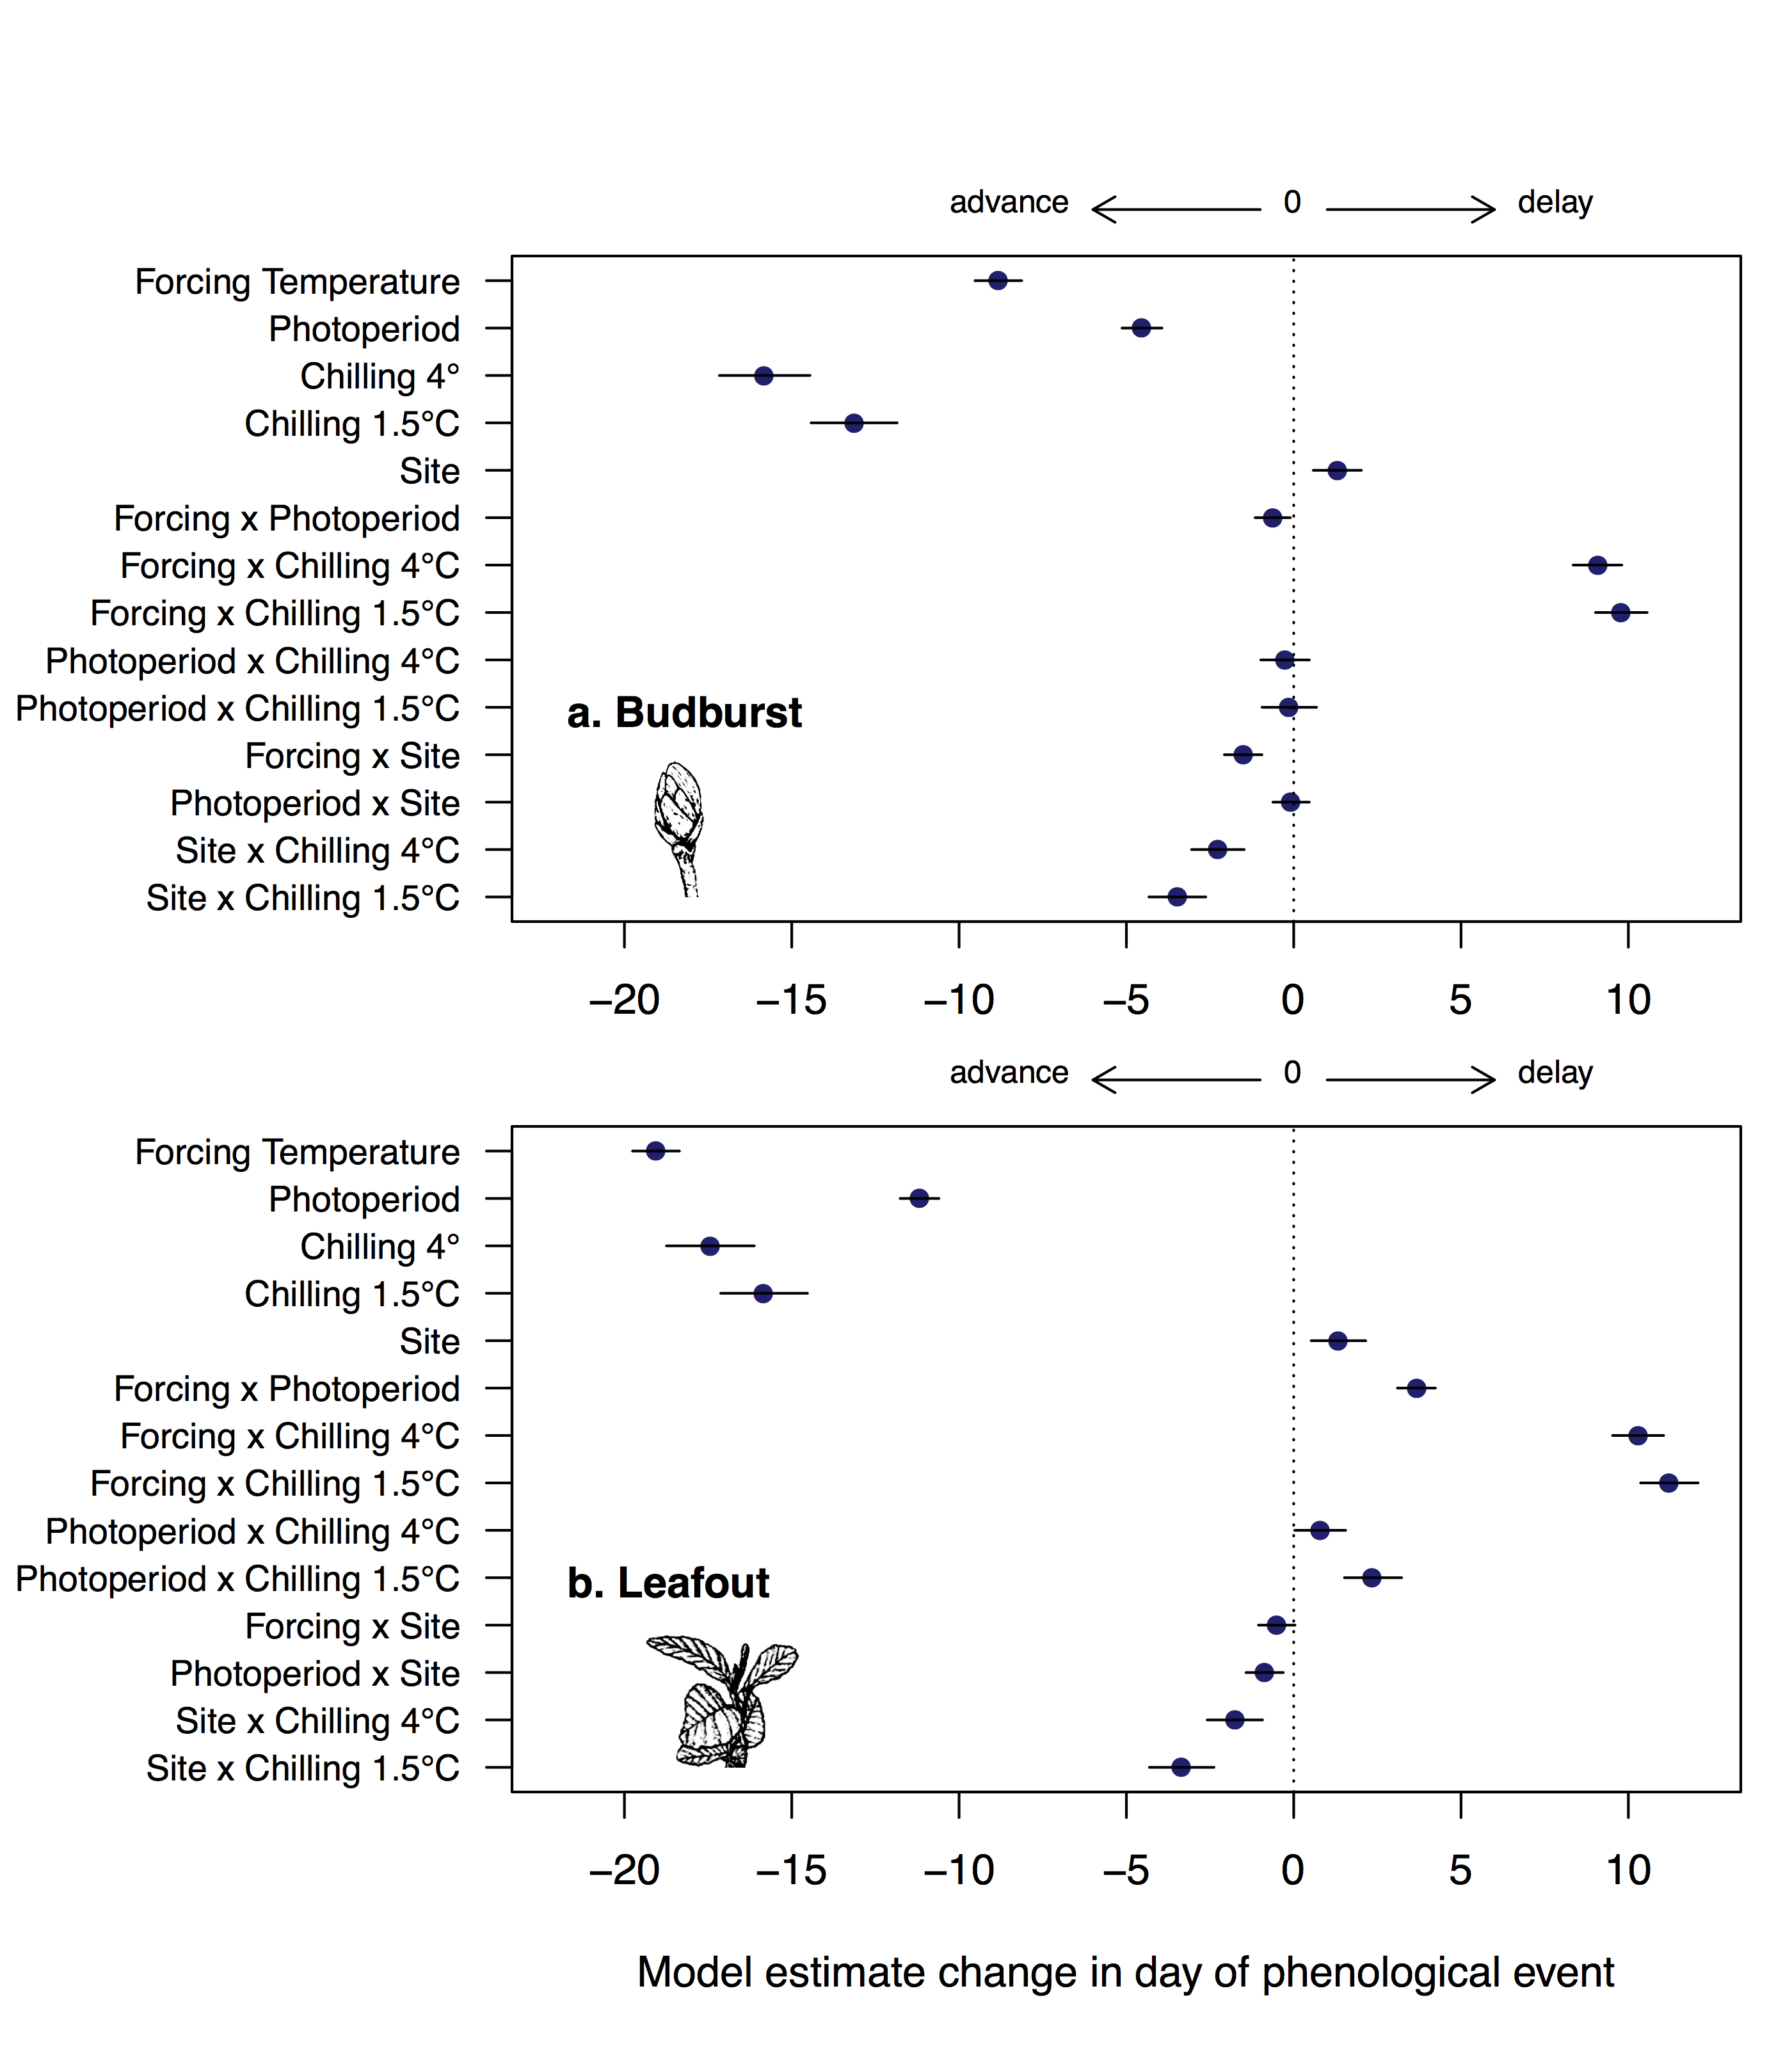
\includegraphics[width=0.9\textwidth]{images/Fig1_bb_lo.png}
\caption{Effects of forcing temperature, photoperiod, chilling and site on budburst (a) and leafout (b) days across 28 species. Dots and bars show mean and 50\% credible intervals from a Bayesian hierarchical model that also incorporated species-level variations (see Tables S2-S3; Figs. 1, S2-S3). Advances in phenology are shown by negative numbers; delays are shown as positive. Forcing temperatures and photoperiods were two levels each (see Methods), and chilling treatments were applied for 30 days. Budburst and leafout images from \citet{Finn:2007}.}
\label{fig:maineff}
\end{figure}

\newpage
\begin{figure}[h!]
\centering
\noindent 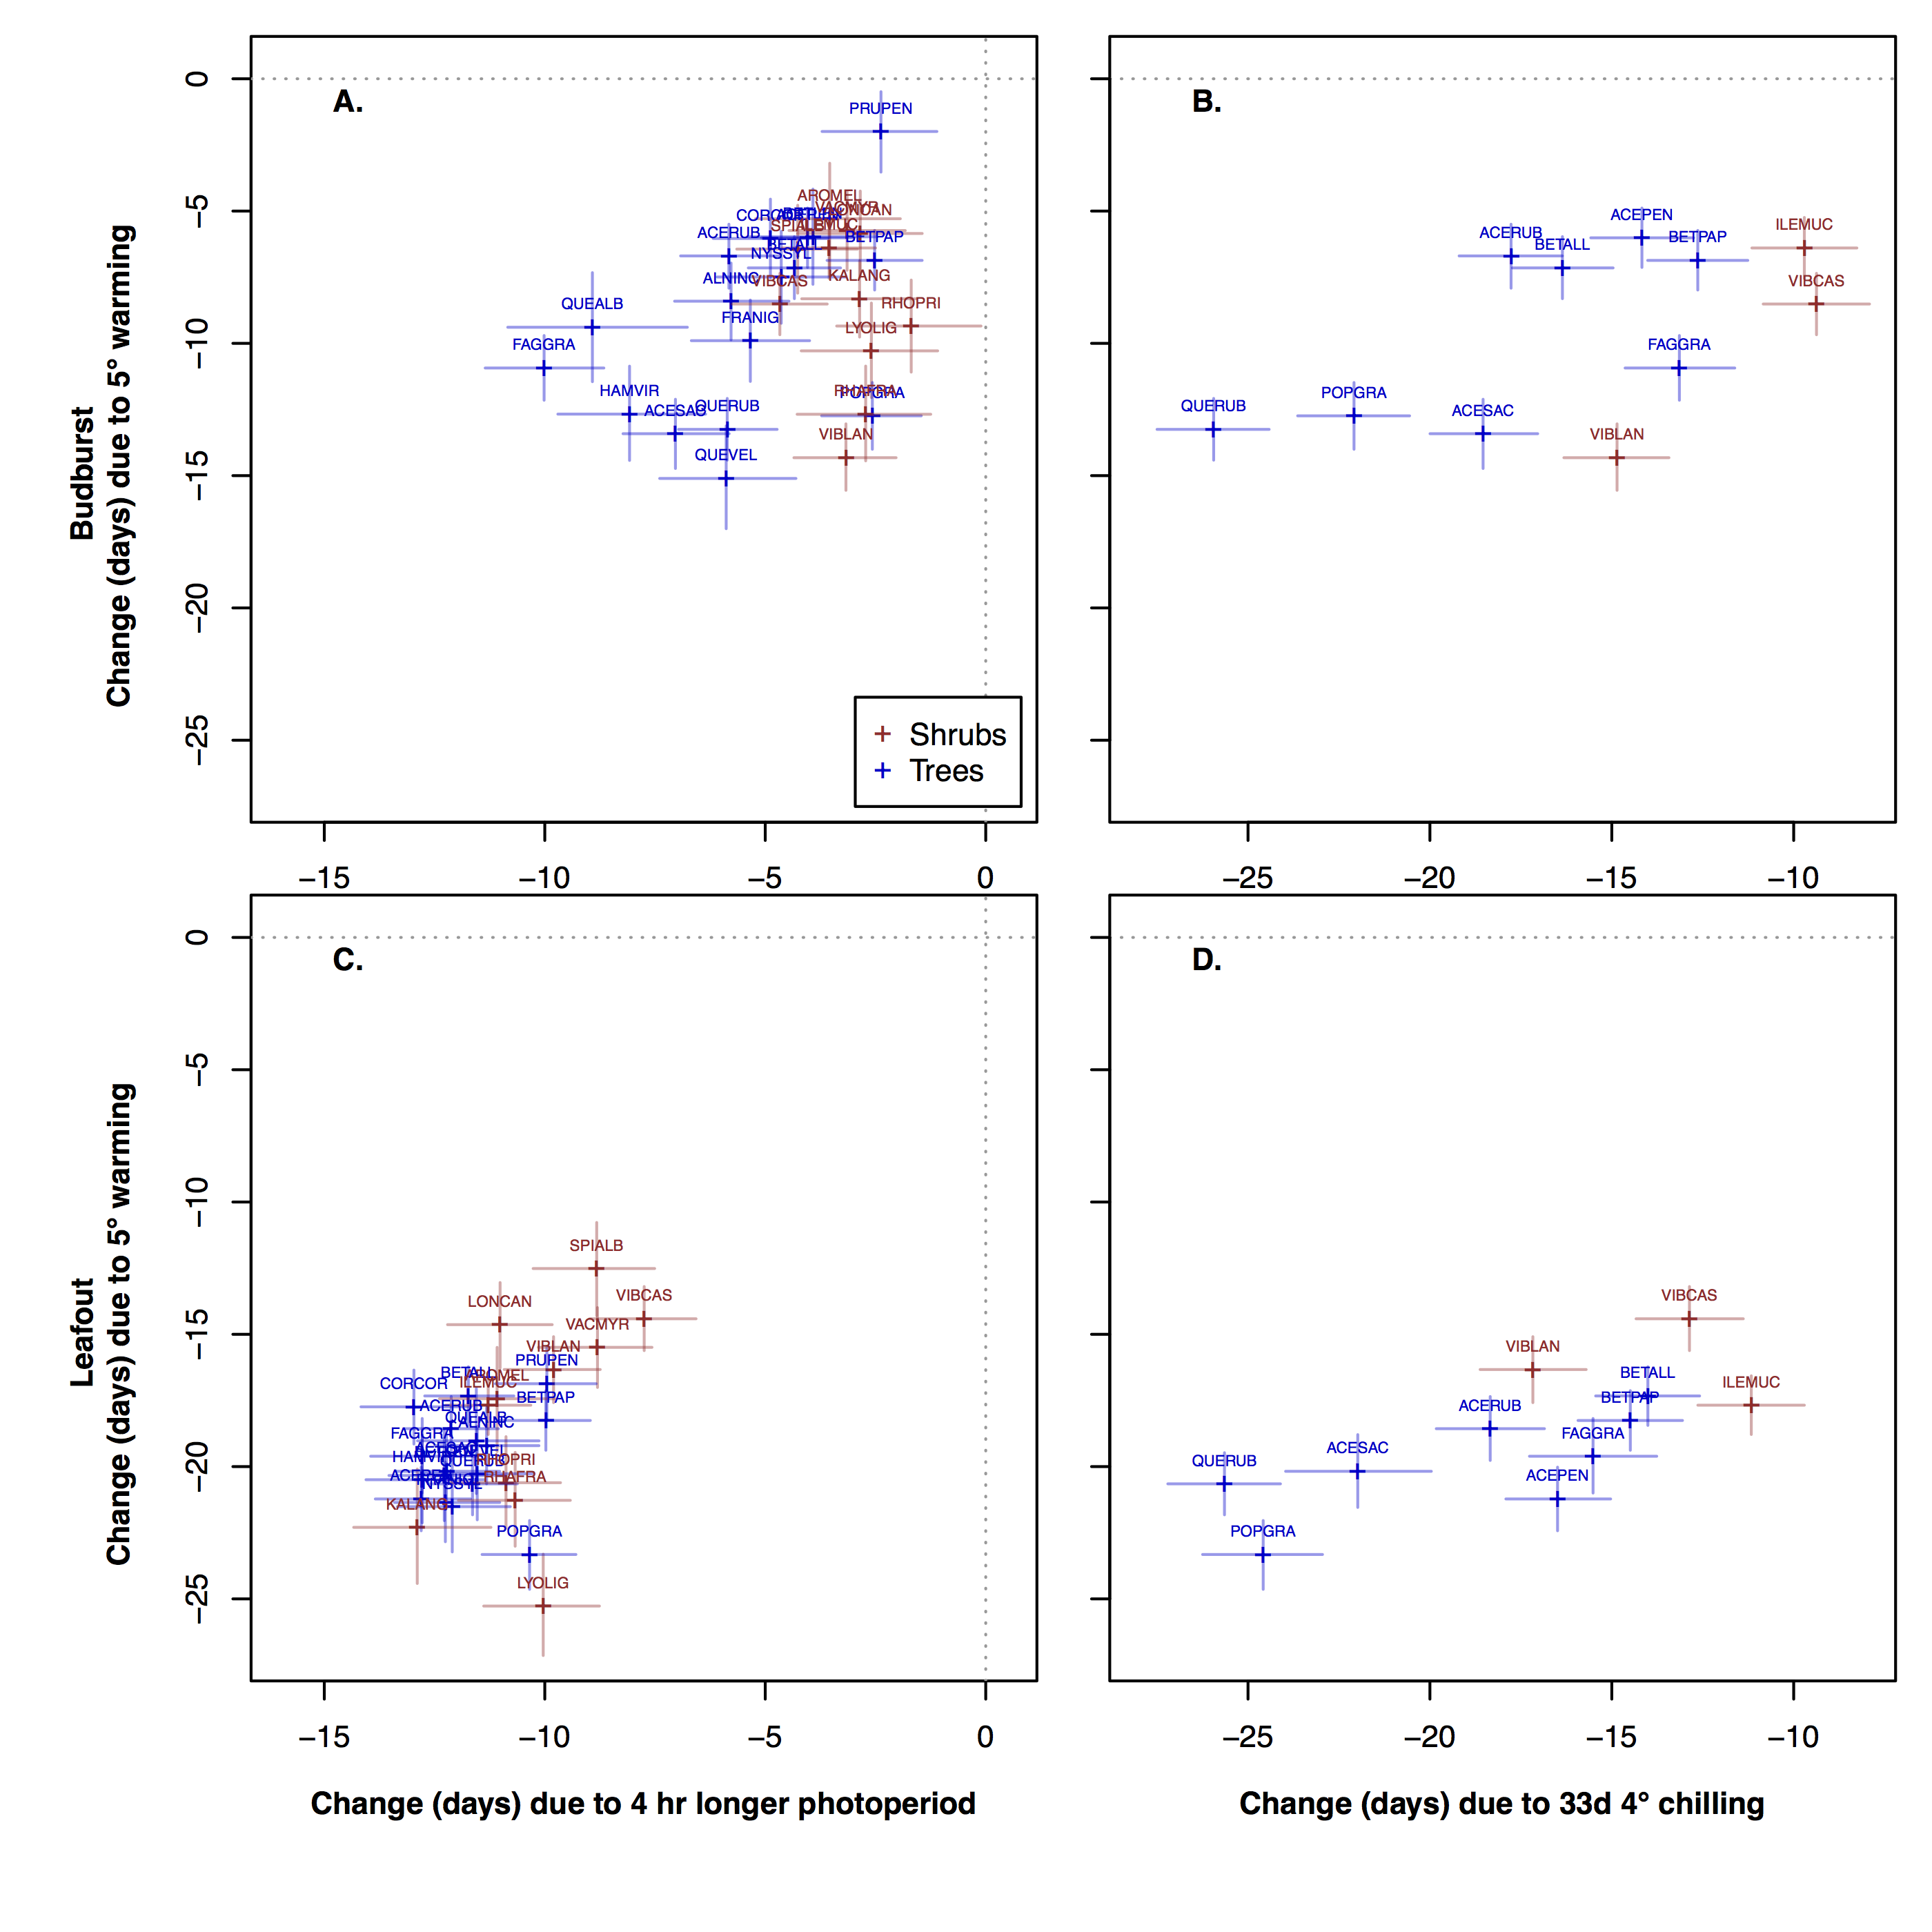
\includegraphics[width=1\textwidth]{images/Fig2_4panel.png}
\caption{Effects of photoperiod, temperature and chilling across species (shrub species shown in red, tree species in blue): Crosses and bars show mean and 50\% credible intervals from a Bayesian hierarchical model (see Tables S2-S3; Figs. 1, S2-S3). For visualization purposes, species names are represented by the first three letters of the genus and first three letters of the species epithet (see Table S1 for full species names and Fig. S5-S6 for additional versions of figure).}
\label{fig:sppeff}
\end{figure}

\newpage
\begin{figure}
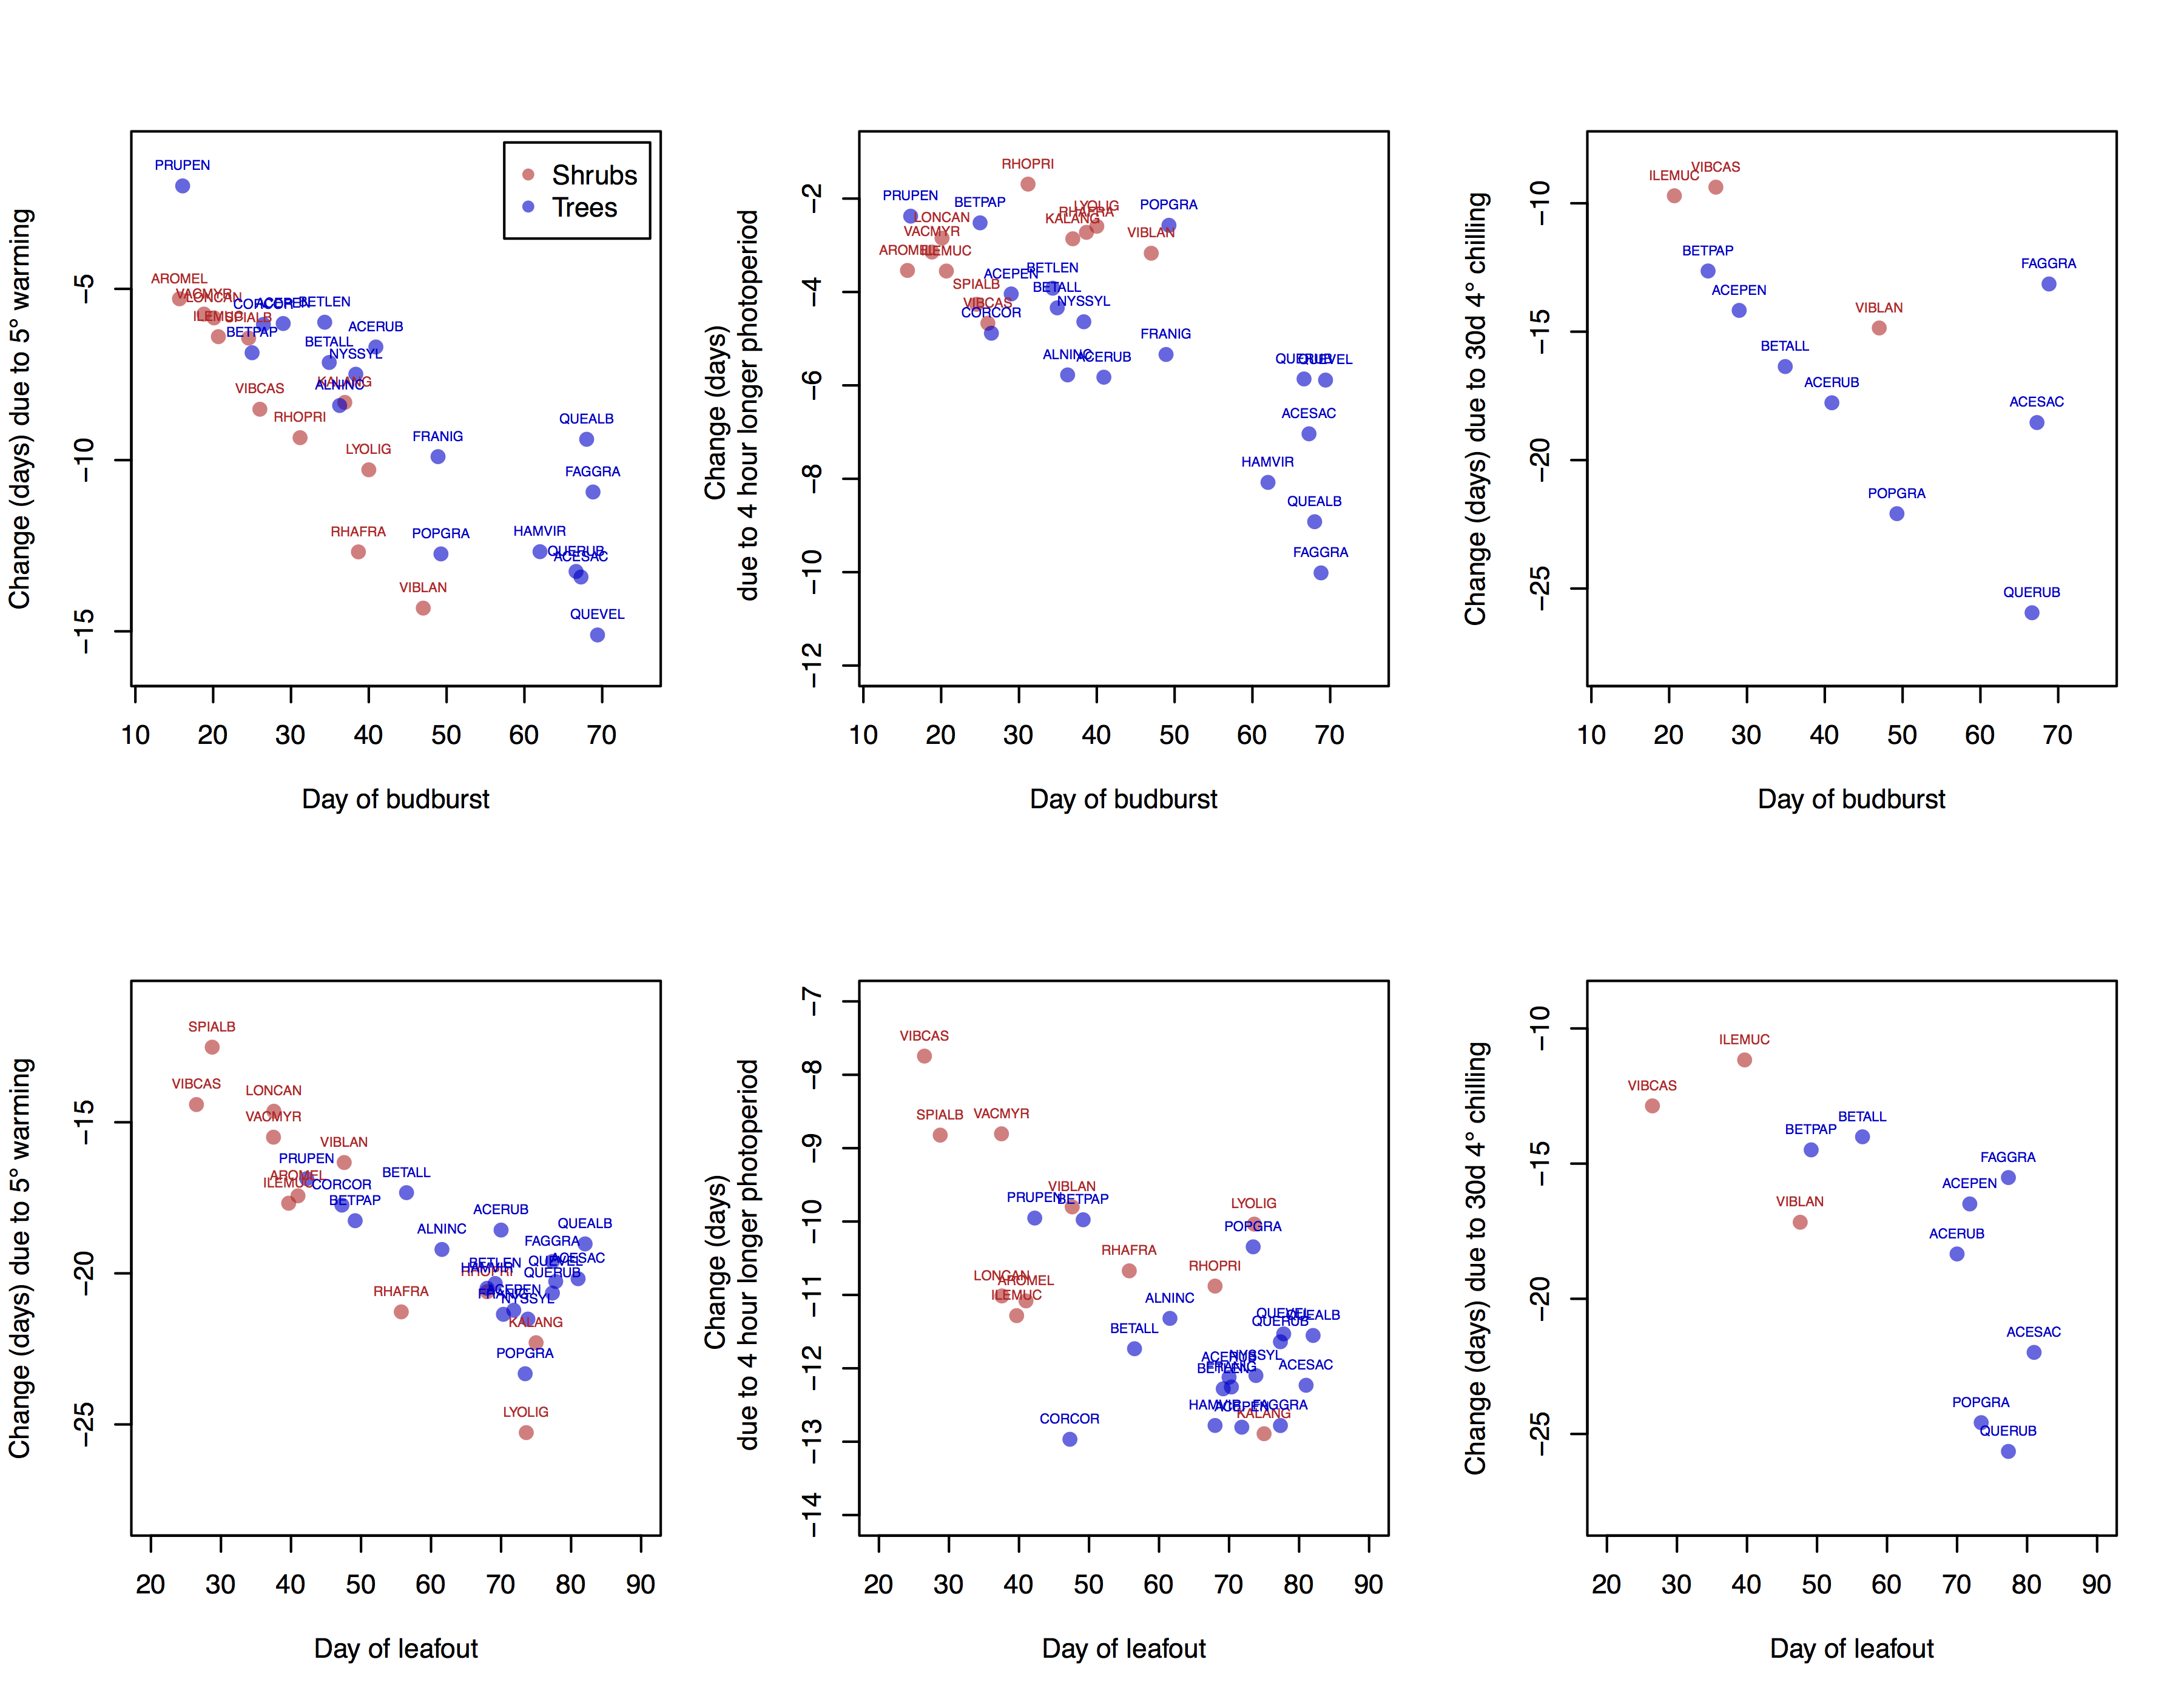
\includegraphics[width=1\textwidth]{Sens_vs_day_treeshrub.png}
\caption{Effects of photoperiod, temperature and chilling across species compared to day of budburst (upper panels) or leafout (lower panels): we show mean estimates of sensitivity to warming, photoperiod, and chilling from a Bayesian hierarchical model (see Tables S2-S3; Figs. 1, S2-S3). For visualization purposes, species names are represented by the first three letters of the genus and first three letters of the species epithet (see Table S1 for full species names).}
\label{fig:commsens}
\end{figure}

%\listoftables
%\listofFig.s

% <<echo=FALSE>>=
% setwd("~/Documents/git/projects/treegarden/budexperiments/analyses")

% source("Pheno Budburst analysis.R")
% @

\end{document}





%%%%%%%% %%%%%%%% %%%%%%%% %%%%%%%% %%%%%%%%% 

%%%%%%%% %%%%%%%% %%%%%%%% %%%%%%%% %%%%%%%%% 
%%%%%%%% START OF ORIGINAL TEXT FROM DAN %%%%%%%%%%%%%
%%%%%%%% %%%%%%%% %%%%%%%% %%%%%%%% %%%%%%%%% 

%%%%%%%% %%%%%%%% %%%%%%%% %%%%%%%% %%%%%%%%% 

A major challenge to build on this extensive study of how temperature and photoperiod drive spring phenology is understanding---and possibly predicting---how the sensitivity to each cue and their interactions varies across species. Temperate woody species are well known to  have different sets of cues, depending on the species \citep{Lechowicz:1984aa,Korner:2010}---with some species showing stronger spring forcing or photoperiod cues, for example. A possible framework for understanding this variation in cues comes from considering how adaptive pressures may drive temperate plant phenology \citep{Wolkovich:2011aa,Wolkovich:2014ab}. Temperate woody plants should aim to maximize the carbon gain that comes from starting growth early in the season and gaining first access to critical resources such as light, soil nitrogen and water, while at once minimizing the risk of tissue loss to frost in early spring \citep{Korner:2010,Gu:2008aa,Hufkens:2012aa}. Across a community of co-occurring species we may expect a diversity of strategies to address these pressures---allowing each species to persist in the community. 

The ways that species manage such risks, and possible rewards, can vary in both when on average in the spring they begin their growth, and also how flexible they are around that average timing. Related to this, two trade-offs have been described for spring phenology of woody plants in response to a variable spring environment: tolerance versus avoidance of freezing \citep{Sakai:1987aa}, and opportunistic versus conservative strategies \citep{Korner:2010}. The former describes how early or late in a season a species leafs out---with tolerant species consistently leafing out early each year, while avoidance species would consistently leaf out late---while the latter describes how flexible a species or individual may be in response to unusually early warm-up events, with opportunistic species tending to have phenological cues that yield variable leaf-out times across variable years and conservative species tending to leaf out consistently across variable years. While related, these tradeoffs predict some differences in the characteristic of the cues and related traits of each species and may combine to produce contrasting changes in phenology. 

Importantly, the combinations of these axes can result in non-intuitive responses at the community level. For example, under a relatively stationary long-term climate early tolerant but conservative species would enjoy the advantage of a long growing season. Yet, as that environment becomes nonstationary---as is the case with climate change---such advantages may quickly eroded. In contrast under a warming environment, species that are relatively late in leafing out (avoidance) and flexible (opportunistic) close the gap with those tolerant species in bud burst and leaf out times. Thus, understanding both the rank order of phenology and the sensitivity of species to environmental cues across a whole community is important in understanding how a changing climate will affect community dynamics. % Opportunistic strategies should benefit species in a nonstationary environment, as in a warming world where mild winters are less an unusual occurrence.

% EMW: Can we say somewhere quickly in below paragraph what the predictions are for phenological cues? It seems like tolerant species would have to have cues to be early (low requirements for everything?) and avoidance species need cues to be late .... If phenological cues for tolerant-avoidance has not been discussed much before we should acknowledge that also. 
For the tolerance-avoidance axis, plants may either tolerate risk of spring freezing in two major ways: through phenological cues that allow them to leaf out well after all frost risk has passed (avoidance) or through investing in tissue which can withstand freezing (tolerant). For perennial plants, it has been found that leaf and wood tissues of species which have later phenologies can be more sensitive to frost damage \citep{CaraDonna:2014aa,Vitasse:2014aa,Lechowicz:1984aa}, supporting the notion of a tradeoff between tolerance and avoidance of freezing risk. In contrast, avoidance-strategy plants would be expected to express lower tissue densities, with the shorter growing season being made up for by faster growth rates, less investment in structural elements of tissue, and relatively greater percent nitrogen in leaves. 

The axis of conservative versus opportunistic strategies makes specific predictions for the phenological cues of differing species and may also predict the related traits of species. In opportunistic plant strategies, temperature is the dominant driver of spring phenology, while for species with conservative strategies, photoperiod and chilling would be the major drivers. It has been found for several cases that short-lived, early successional species typically exhibit such opportunistic strategies, and late-successional species are more typically chilling- and photoperiod-controlled in breaking of dormancy \citep{Korner:2010,Caffarra:2011ab,Basler:2012aa}.

% would like to find a citation for changes in traits within early part of growing season, have not found this.
% other timing and traits: earlier phenology, fleshy fruits \citep{Kjell-Bolmgren:2005aa}, even after doing PIC
% For herbaceous species, two axes: early vs late, and fast vs slow growth. Early-fast, late-slow, late-fast all possible \citep{Sun:2011aa}. Early-fast related to short stature and high relative groth rate

Tests of how these two tradeoff axes drive phenology across a co-occurring community of species have not previously been carried out. As the abiotic environment is not the sole contributor to plant performance, considering a suite of co-occurring species together is key for making progress in understanding the role phenology plays in shifts in community composition and ecosystem functioning \citep{Cleland:2007aa}.

To test the interactive effects of the three controlling drivers of spring phenology, temperature, photoperiod, and chilling across latitudes, we carried out a study of 28 woody plants. We assessed both bud burst and leaf-out to account for the potential different sensitives of these phenological stages to abiotic drivers, and analyzed responses across all species to examine the support for how well the tolerance-avoidance and opportunistic-conservative tradeoff axes represent temperature plant spring phenology.

%%%%%%%%%%%%%%%%%%%%%%%%%%%%%%%%%%%%
\section*{Results}
%%%%%%%%%%%%%%%%%%%%%%%%%%%%%%%%%%%%

Major findings
\begin{itemize}
\item{All of the 28 species showed sensitivity to all three of the abiotic drivers.}
\item{The strength of the sensitivity to each driver was coordinated, not showing a trade-off axis}
\item{Species with greater sensitivity were generally later-phenology, canopy trees, rather than early-season, early-successional shrubs.}
\end{itemize}

Forcing temperature, photoperiod, and chilling individually and interactively determined timing of both bud burst and leaf-out. We found photoperiod sensitivity was common and strong across all of the woody plants studies, consistently reducing time to phenological responses for each species, across sites of origin. 

For the 28 species studied, sensitivity to temperature and photoperiod cues for leaf-out times varied substantially, and---in contrast to our hypotheses [that we set up in the intro]---co-varied overall. The coordinated response to warming temperatures and longer photoperiod was consistent with overall pace of phenological events; earlier-leafing out species (namely the shrubs \emph{Spiraea alba}, \emph{Viburnum cassanoides}, and \emph{Vaccinium myrtilloides}) exhibited relatively limited advances to either warming or longer days, while later leafing-out species showed ability to advance their phenology by in response to both warming and longer days. Thus, no trade-off was observed between photoperiod-cued and temperature-cued species, but rather species exhibit coordinated responses to both environmental factors (Fig. \ref{fig:maineff}). 

While both photoperiod and temperature cues were important for driving woody plant phenology, responses to chilling were also substantial. Bud burst day was accelerated most by the chilling treatments. Tables 1 and 2 summarizes hierarchical mixed-effects model analysis of day of bud burst and leaf-out, with negative values indicate earlier day of experiment for each event. Overall the 5\degree C experimental warming resulted in 6.8 days earlier bud burst and 21.9 days earlier leaf out. Such advance was delayed by the each chilling treatment, as indicated by the positive coefficient for the temperature x chilling interactions. Latitude of origin (Site) overall had little direct effect on bud burst or leaf-out, but populations from the northern site tended to exhibit slower bud burst and leaf-out, with a more rapid bud burst and leaf out in response to the chilling treatments (indicated by negative coefficients for site x chilling treatments).

Warming, photoperiod, and chilling individually and interactively acted to drive bud burst and leaf out earlier across species. The strength of the acceleration in bud burst due to both warming and photoperiod were similar, but the acceleration of leaf out due to warming exceeded that of photoperiod for both phenological stages. Surprisingly, site of origin exerted limited effect on either bud burst or leaf out across species. 

\subsection*{Effect of chilling}
Species varied widely in response to chilling treatments, with some exhibiting strong chilling requirements (\emph{Acer saccharum}, \emph{Fagus grandifolia}), while others exhibited little change in phenological advancement under experimentally manipulated chilling. Overall, bud burst and leaf-out advanced by 22.1 or 26.4 days under additional 30 d of vernalization at 4\degree C, and advanced by a reduced amount of 19.7 or 26.1 days under 30 d of vernalization at 1.5\degree C. The reduced chilling effect at the lower temperature chilling is consistent with the Dynamic Model of chilling accumulation. % And also consistent with the Utah model?

Species-specific responses to chilling demonstrate that chilling requirements are not uniform across species, with 
of \emph{Fagus grandifolia} to increasingly strong vernalization varies by latitude of origin and by phenological stage; winter chilling reduced day to bud burst and leaf-out, but more strongly for individuals from the northern site.

While nearly all species showed advances in spring phenology in response to the experimental chilling treatment, as indicated by fewer days to phenological events for the 4\degree C and 1.5\degree C treatments, the majority of species (e.g. \emph{Populus grandidentata}) showed delays in both bud burst and leaf out at the more severe chilling treatment. Of the species exposed to the additional chilling, only \emph{Fagus grandifolia} was consistently advanced by the more severe chilling.

\subsection*{Species-specific responses}

Species traits partly explain variation in warming and photoperiod sensitivities of leaf out. Plants with high nitrogen leaves, as well as high SLA (thinner, less dense) leaves, were significantly later in both bud burst and leaf out. Thus early leaf out species tended to be tougher, less N-dense, and have higher carbon investments than later species. Greater wood density had inconsistent effects as a driver, with higher wood density driving later bud burst but tending to drive earlier leaf out.

Ring-porous species (\emph{Fraxinus sp.}, \emph{Lonicera}, \emph{Myrica}, and \emph{Quercus}; lower values of Pore Anatomy variable) exhibited significantly later bud burst and leaf out compared to diffuse-porous species, in line with previous work on wood anatomy and freezing risk \citep{Sperry:1992}.

Shrubs with low specific leaf area (thick/dense leaves) and high stem density were more likely to leaf out earlier. For trees, with an overall later leaf out pattern, 

Rank order of leaf out and bud burst was stable across warming and photoperiod treatments. Chilling treatments shifted the order, for example \emph{Fagus grandifolia} was the 23-28th species to burst bud with no additional chilling, but advanced to the 10-11th species to burst bud in with additional chilling. Within chilling treatments, the consistency of the rank order was high, with standard deviation of the rank order ranging from 2.05 d (bud burst, no additional chilling) to 0.75 d (leaf out, additional chilling at 4\degree C). Compared to field observations, rank order of leaf out was generally most related in the cool, short-day treatment with no additional chilling (Fig. S10).

%%%%%%%%%%%%%%%%%%%%%%%%%%%%%%%%%%%%
\section*{Discussion}
%%%%%%%%%%%%%%%%%%%%%%%%%%%%%%%%%%%%

Photoperiod sensitivity is common in northeastern woody plants, and greater photoperiod sensitivity is related to, not instead of, temperature sensitivity. Taken together, this result shows that the opportunism-conservatism tradeoff is not supported by the data for this suite of species. The most sensitive species to both cues, namely the species which could advance their phenology in response to both longer days and warmer temperatures, were the later-successional tree species, rather than the shrubs. The trait data indicate partially that the species earliest to leaf out, namely the shrubs and small trees, also had lower SLA and lower leaf \%N, indicating greater investment in tissue structures. These results support the tolerance-avoidance tradeoff, with the early phenology species being tolerant to freezing but relatively less able to advance their phenology in a warming environment. These results also indicate that the later-successional species have potentially the most to gain from a warming world, as they can extend their growing seasons  

While both photoperiod and temperature sensitives were common, chilling sensitivity greatly outweighed both of these factors. It is important to note that the results from the chilling part of this experiment are derived from 11, not 28 species, but the strength of this effect is notable. Strong chilling requirements were detected both for bud burst and leaf out responses, and the most substantial advance in spring phenology came from the more mild chilling treatment, at 4\degree C, with reduced effectiveness of chilling at 1.5\degree C. 

These three factors did show some degree of substituability, meaning for example that a lack of chilling could be made up for by an increase in temperature. These are indicated by the positive two-way interactions; chilling and forcing temperature are more substitutable than chilling and photoperiod, for both bud burst and leaf out.

We found only limited support for the northern populations showing more conservative (photoperiod-cued) strategies in these 28 species was found, with small delays in both phenological events for populations from the more northern site. The latitudinal range studied here is within the range of the phenotypic flexibility of these species. Of these study species, we should not be overly concerned about being photoperiod limited at the more northern sites; given sufficient pace of dispersal, they will be able to track a changing climate.

bud burst is sensitive to the same environmental cues as leaf out, but species show idiosyncratic orderings of their sensitivity to environmental cues at these two phenological stages; leaf out responses can not necessarily be used to back-cast bud burst responses. Bud burst showed a more limited total response to environmental cues, and species were more tightly clustered in those responses.

Surprisingly, the smaller statured, earlier-leafing out shrubs and small trees exhibited reduced sensitivity to all three factors of temperature, photoperiod, and chilling. They are relatively more fixed in their timing of both bud burst and leaf out, perhaps indicating an alternative mechanism for timing of spring phenology in these plants \citep{Pagter:2015}.

Given these results, the future of the northeastern forests may shift towards later-phenology, canopy trees, as these species demonstrated a greater ability to lengthen their growing seasons opportunistically in response to warmer temperatures.
% I think we should be more cautious in stating this. We still don't know *what* controls their leaf out! -- I think we can make some educated guesses here!

% Re the above about shrubs versus trees -- I am just not sure what to think! And it comes back to the models. Our models give each species a fundamental leaf out day -- their intercept. This makes lots of sense to me but biologically I am not sure what to do with it (and if we take it away then the early species become hyper-sensitive, right? - right). I think we need to think on what that intercept means and what we should and shouldn't say given that it's in our models. I think it could be what you suggested, it could also be that they have super weak chilling, it could be that they are sensitive to humidity or something we don't study. But fundamentally I think we need to think harder about that before we push our conclusions too far. 


%%%%%%%%%%%%%%%%%%%%%%%%%%%%%%%%%%%%%%%%%
%%%%%%%% END OF ORIGINAL TEXT FROM DAN %%%%%%%%%%%%%
%%%%%%%%%%%%%%%%%%%%%%%%%%%%%%%%%%%%%%%%%



%%%%%%%%%%% Fig.s
% 1. Experimental design

% 2. model output
\begin{Fig.}
\begin{center}
\caption{Modeled effects plots, bud burst and leaf out}
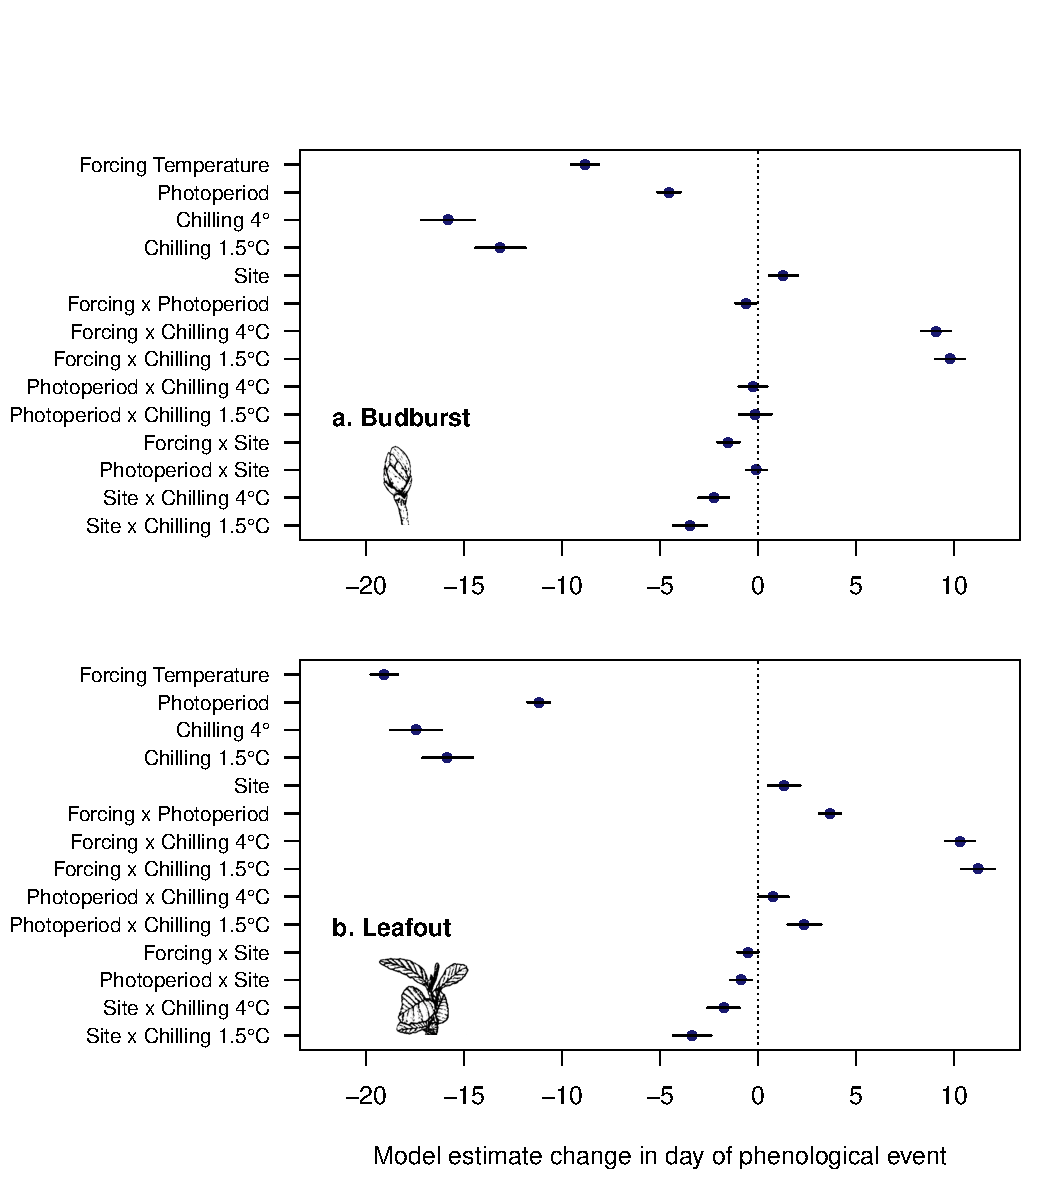
\includegraphics[scale=0.8]{Fig1_bb_lo}
\label{fig2}
\end{center}
\end{Fig.}

% 3. Temp + Pheno + Chill sensitivity

\begin{Fig.}
\caption{Sensitivity of bud burst and leaf out to warming, leaf out, and chilling.}
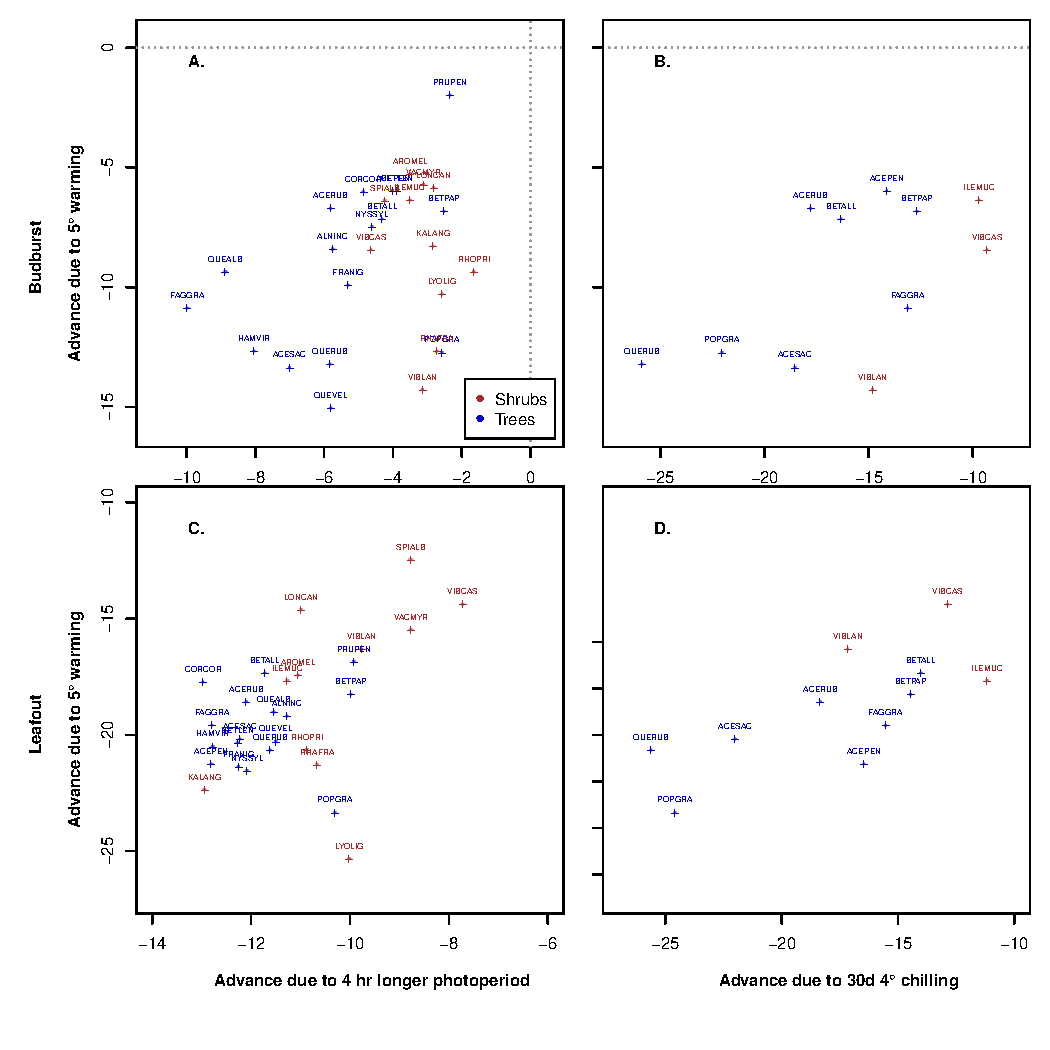
\includegraphics[scale=0.9]{Fig2_4panel}
\label{fig3}
\end{Fig.}

\end{document}}



%%%%%%%%%%%%%%%%%%%%
%%%%%%% EDITS %%%%%%%%%
%%%%%%%%%%%%%%%%%%%%

% Lizzie's original attempt to write just results (14 May 2017):
In total we monitored XX clippings and took XX observations of phenology (budburst and leafout as assessed by the BBCH scale) in an experiment that ran XX days. Higher forcing temperatures, longer photoperiod, and more chilling all caused large advances in budburst and leafout (Fig. \ref{fig:maineff}). The effects of forcing and chilling temperatures offset one another, as shown by their interactive delayed response (Fig. \ref{fig:maineff}). The two forest sites showed very similar responses, with only a minor delay in overall timing for the more northern site (Fig. \ref{fig:maineff}) and a more pronounced effect site through its interaction with chilling (ADD). We found responses to more colder (1.5C) chilling was similar or more muted compared to responses to a higher temperature (4C) of chilling (Fig. \ref{fig:maineff}-2).\\

At the community level we found that all species showed all three cues: every species we studied was responsive to forcing temperatures, photoperiod and chilling (SuppFig). In contrast to our expectations that within species cues would trade off, we found that species tended to show coordinated cues, especially between forcing and photoperiod (Fig. \ref{fig:sppeff}). Thus, a species with a strong response to forcing temperature generally also had a strong response to photoperiod, and similarly a species with a comparatively weak response to forcing also had a weaker response to photoperiod. This was also seen somewhat with chilling (Fig. \ref{fig:sppeff}), though we have fewer species with which to assess the relationship (see Methods). \\

Responses to cues were qualitatively similar across both budburst and leafout, but quantitatively varied greatly between the two phenophases (Fig. \ref{fig:maineff}-2), with responses generally greater to leafout (Fig. \ref{fig:maineff}). This change was dramatic for the response to forcing and photoperiod where the result changed XX from budburst to leafout (Fig. \ref{fig:maineff}, Table SX). The order of magnitude of species responses also shuffled between the two stages (Fig. \ref{fig:sppeff}). For example, shrubs tended to show weaker photoperiod effects to budburst (Fig. \ref{fig:sppeff}a) but this was not seen as consistently in the response to leafout (Fig. \ref{fig:sppeff}c). 

%%% From the intro: 

% Traits/strategies
Physiologically, tolerance to freezing is driven by resistance to rupturing of biomembranes, and is related to dehydration stress \citep{Larcher:2005aa}. 

Different phenological stages may be driven by different environmental cues. The period between bud burst and leaf out is critical for leaf development, as this is a period when plants are highly sensitive to damage from late freezing events, with freezing resistance increasing as leaves expand \citep{Sakai:1987aa}.

Drought-tolerance, which can be related to freezing-tolerance in the ability to resist cavitation, has been show to relate to low wood density in a semi-arid forest, with low-wood density species having increased ability to store water in the dry season and ability to flush leaves in the dry season \citep{Lima:2010aa}. Similarly, for temperate deciduous trees, experimental warming has been shown to both increase total growing season length for species which have higher specific leaf area \citep{Xu:2009aa}. Finally, for deciduous trees, traits can exhibit variation in expression over the growing season, with higher leaf tissue density and allocation of nitrogen following cessation of growth in late summer \citep{McKown:2013aa}.

% Community angle
Temporal separation in resource use is an important driver of plant species coexistence \citep{Mason:2013aa} and such temporal separation can drive ecosystem properties such as biomass accumulation \citep{Sapijanskas:2014aa}, thus understanding both the current order of phenology for co-occurring species and propensity to change in future climates is an important goal of plant phenology science.

% Why do cuttings: can manipulate abiotic conditions on same individual, species specific, can detect early events with more precision than larger-scale studies
Knowing species-specific sensitives of temperate plant phenology to chilling and forcing alone can predict regional-scale phenology \citep{Chuine:2000}. Substantial variation exists at the species level in the magnitude of the temporal advance of spring phenology \citep{Primack:2009aa}, such that the presence of species highly sensitive to temperature change can strongly drive community-level phenology \citep{Diez:2012}.

% Latitude
Factors driving spring phenology include chilling temperatures, photoperiod, forcing temperatures, and latitude of origin. Of these factors, the role of latitude in determining spring phenology has largely been investigated in single-species studies across many sites. Given sufficient distance, more pole-ward sites have lower minimum annual temperatures and shorter growing seasons, making accurate timing of spring phenology even more important. Since day length differences from winter to spring are also greater for higher latitudes, populations of northern plants may be expected to rely more on photoperiod as a cue for spring phenology.

For temperate trees, species can be limited at their northern range by inability to develop mature fruit in a given growing season, while limited at their southern range by inability to break dormancy due to insufficient chilling \citep{Chuine:2010}. Thus phenology can drive range limits. Common garden studies have shown that southern-adapted species, when translocated to a more northern location, exhibit later leaf out compared to species adapted to northern sites \citep{Zohner:2014aa}. If species remain relatively fixed in their timing of leaf out, then northward migration of such late-phenology species may act to counteract community-wide advances in phenology under a warming climate. 

% photoperiod
Photoperiod has long been known to be a critical driver of the onset of endodormancy, in combination with cooling temperatures \citep{Foley:2009aa}. However, the role of photoperiod in determining the breaking of dormancy has been debated, with various authors finding that the strength of day length as a driver may depend on phenological stage, species and location \citep{Heide:1993,Falusi:1996aa}. 

In the few experimental studies that have directly manipulated both forcing temperature and photoperiod, photoperiod has been shown to act to moderate advances in phenology due to warming, with reduced advances due to temperature when day length was short \citep{Heide:1993b,Sanz-Perez:2009aa}. 
% look for additional refs showing non-additive effects (replacability)

% Chilling
% points to make: chilling is a strategy to make sure bud burst/leaf out do not occur too early. This can be a supplemental stragety in addition to photoperiod and temperature cues for breaking endodormancy. [notes to myself: endodormancy: short days in fall. Broken by chilling. Ecodormancy: broken by temperature.

In addition to photoperiod, winter chilling requirements also act as a conservative strategy to avoid damage from early spring freezing, allowing woody plants to avoid breaking bud during unusually early warm spells \citep{Ghelardini:2010aa}.

Chilling requirements are known to vary substantially across species, with some needing relatively little winter chilling to initiate bud burst, and others not bursting bud even in long-day, warm environments unless sufficient chilling has taken place \citep{Korner:2010}. 



